\documentclass[12pt,letterpaper]{article}

\usepackage{amsmath, amsthm, amsfonts, amssymb}
\usepackage{microtype, parskip, graphicx}
\usepackage[comma,numbers,sort&compress]{natbib}
\usepackage{lineno}
\usepackage{longtable}
\usepackage{docmute}
\usepackage{caption, subcaption, multirow, morefloats, rotating}
\usepackage{wrapfig}
\usepackage{hyperref}

\frenchspacing

\begin{document}

\section{Model adequacy}

The in-sample model comparisons are for determining their relative adequacy, or a model's ability to represent the data it was fit to. Comparison between the posterior predictive estimates of in-sample AUC for each of the four models demonstrates that, overall, all of the models have approximately equal in-sample performance (Fig. \ref{fig:auc_hist}). The parameter rich ``past and vary'' model has the greatest median in-sample AUC when compared to the other three models, but there is substantial overlap in their posterior distributions. Additionally, while our parameter rich ``past and vary'' model is possibly the most adequately performing model, the difference or improvement to performance is minimal at best -- all four models have approximately equal in-sample AUC posterior distributions. All of the in-sample AUC estimates from our models are concentrated around an AUC of 0.77 which is interpreted as ``fine but not good'' performance. It is then hard to conclude that there is one ``best'' model which we can rely upon. 
% ROC model comparison
\begin{figure}[ht]
  \centering
  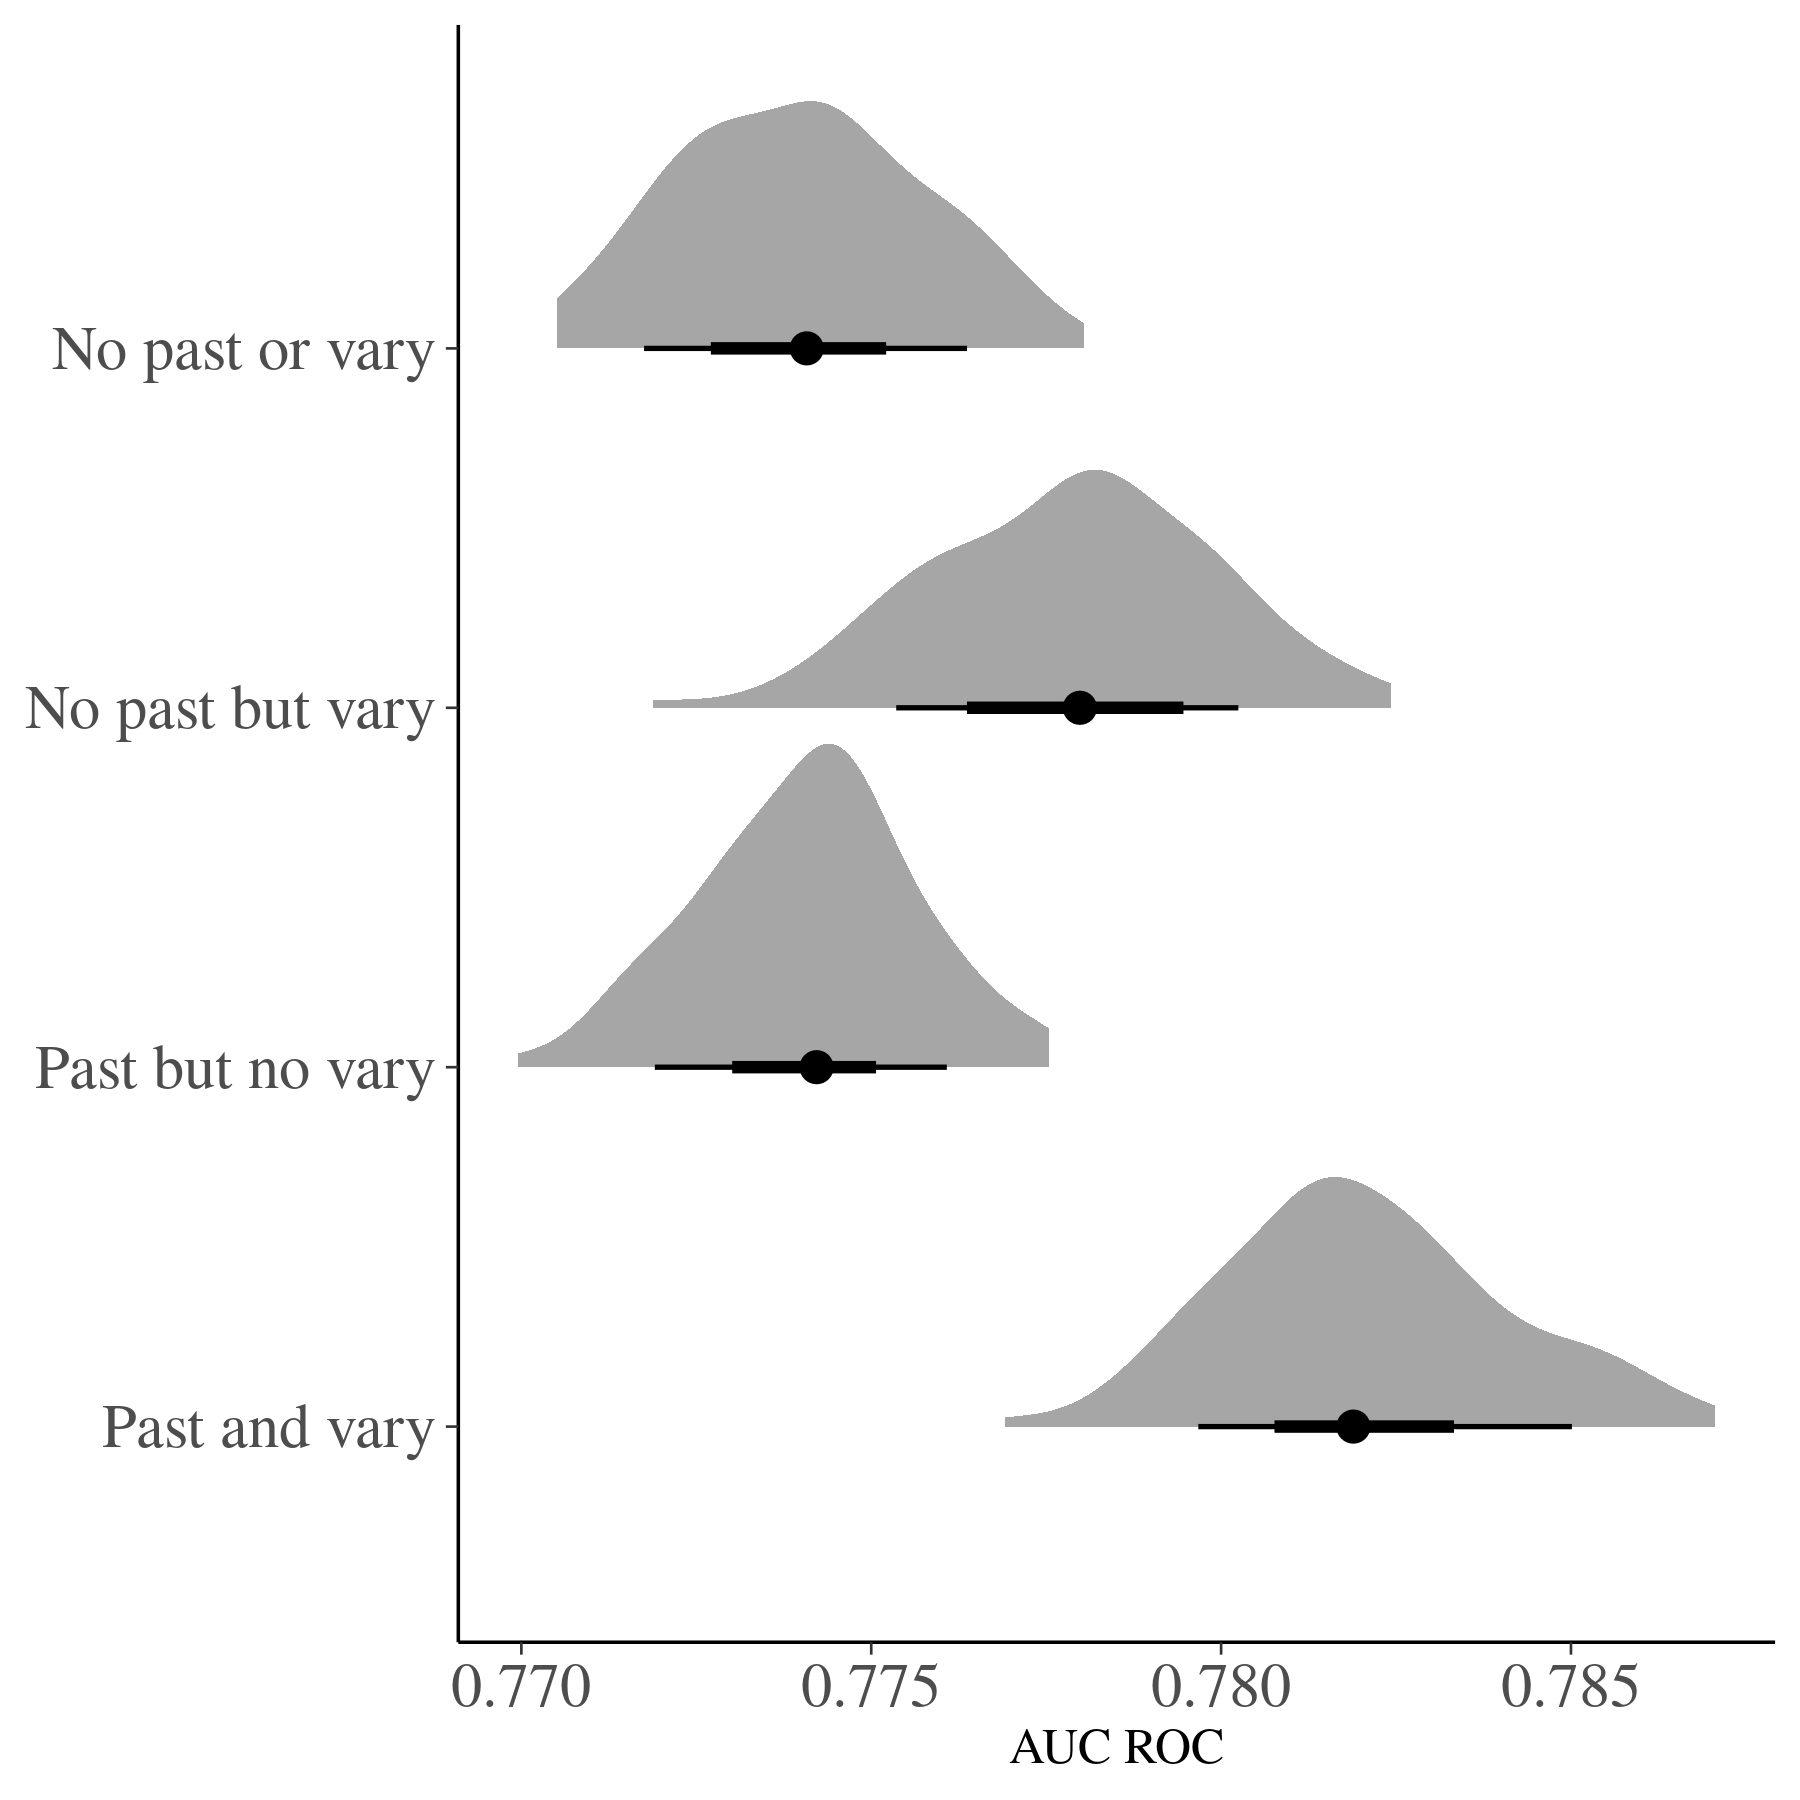
\includegraphics[width=\textwidth,height=0.5\textheight,keepaspectratio=true]{../results/figure/auc_hist}
  \caption{Posterior predictive AUC estimates for each of the four models being compared. These estimates are calculated from each of the models posterior predictive distribution compared to the empirical values. Models with a higher AUC values indicate better performance over models with lower AUC values. AUC is bounded between 0.5 and 1.}
  \label{fig:auc_hist}
\end{figure}


When the posterior predictive distributions of the in-sample AUC estimates are presented over time, the similarity in adequacy between the models becomes more apparent (Fig. \ref{fig:auc_ts}). There are few major or obvious differences in model adequacy between the four models.
% ROC model comparison time series
\begin{figure}[ht]
  \centering
  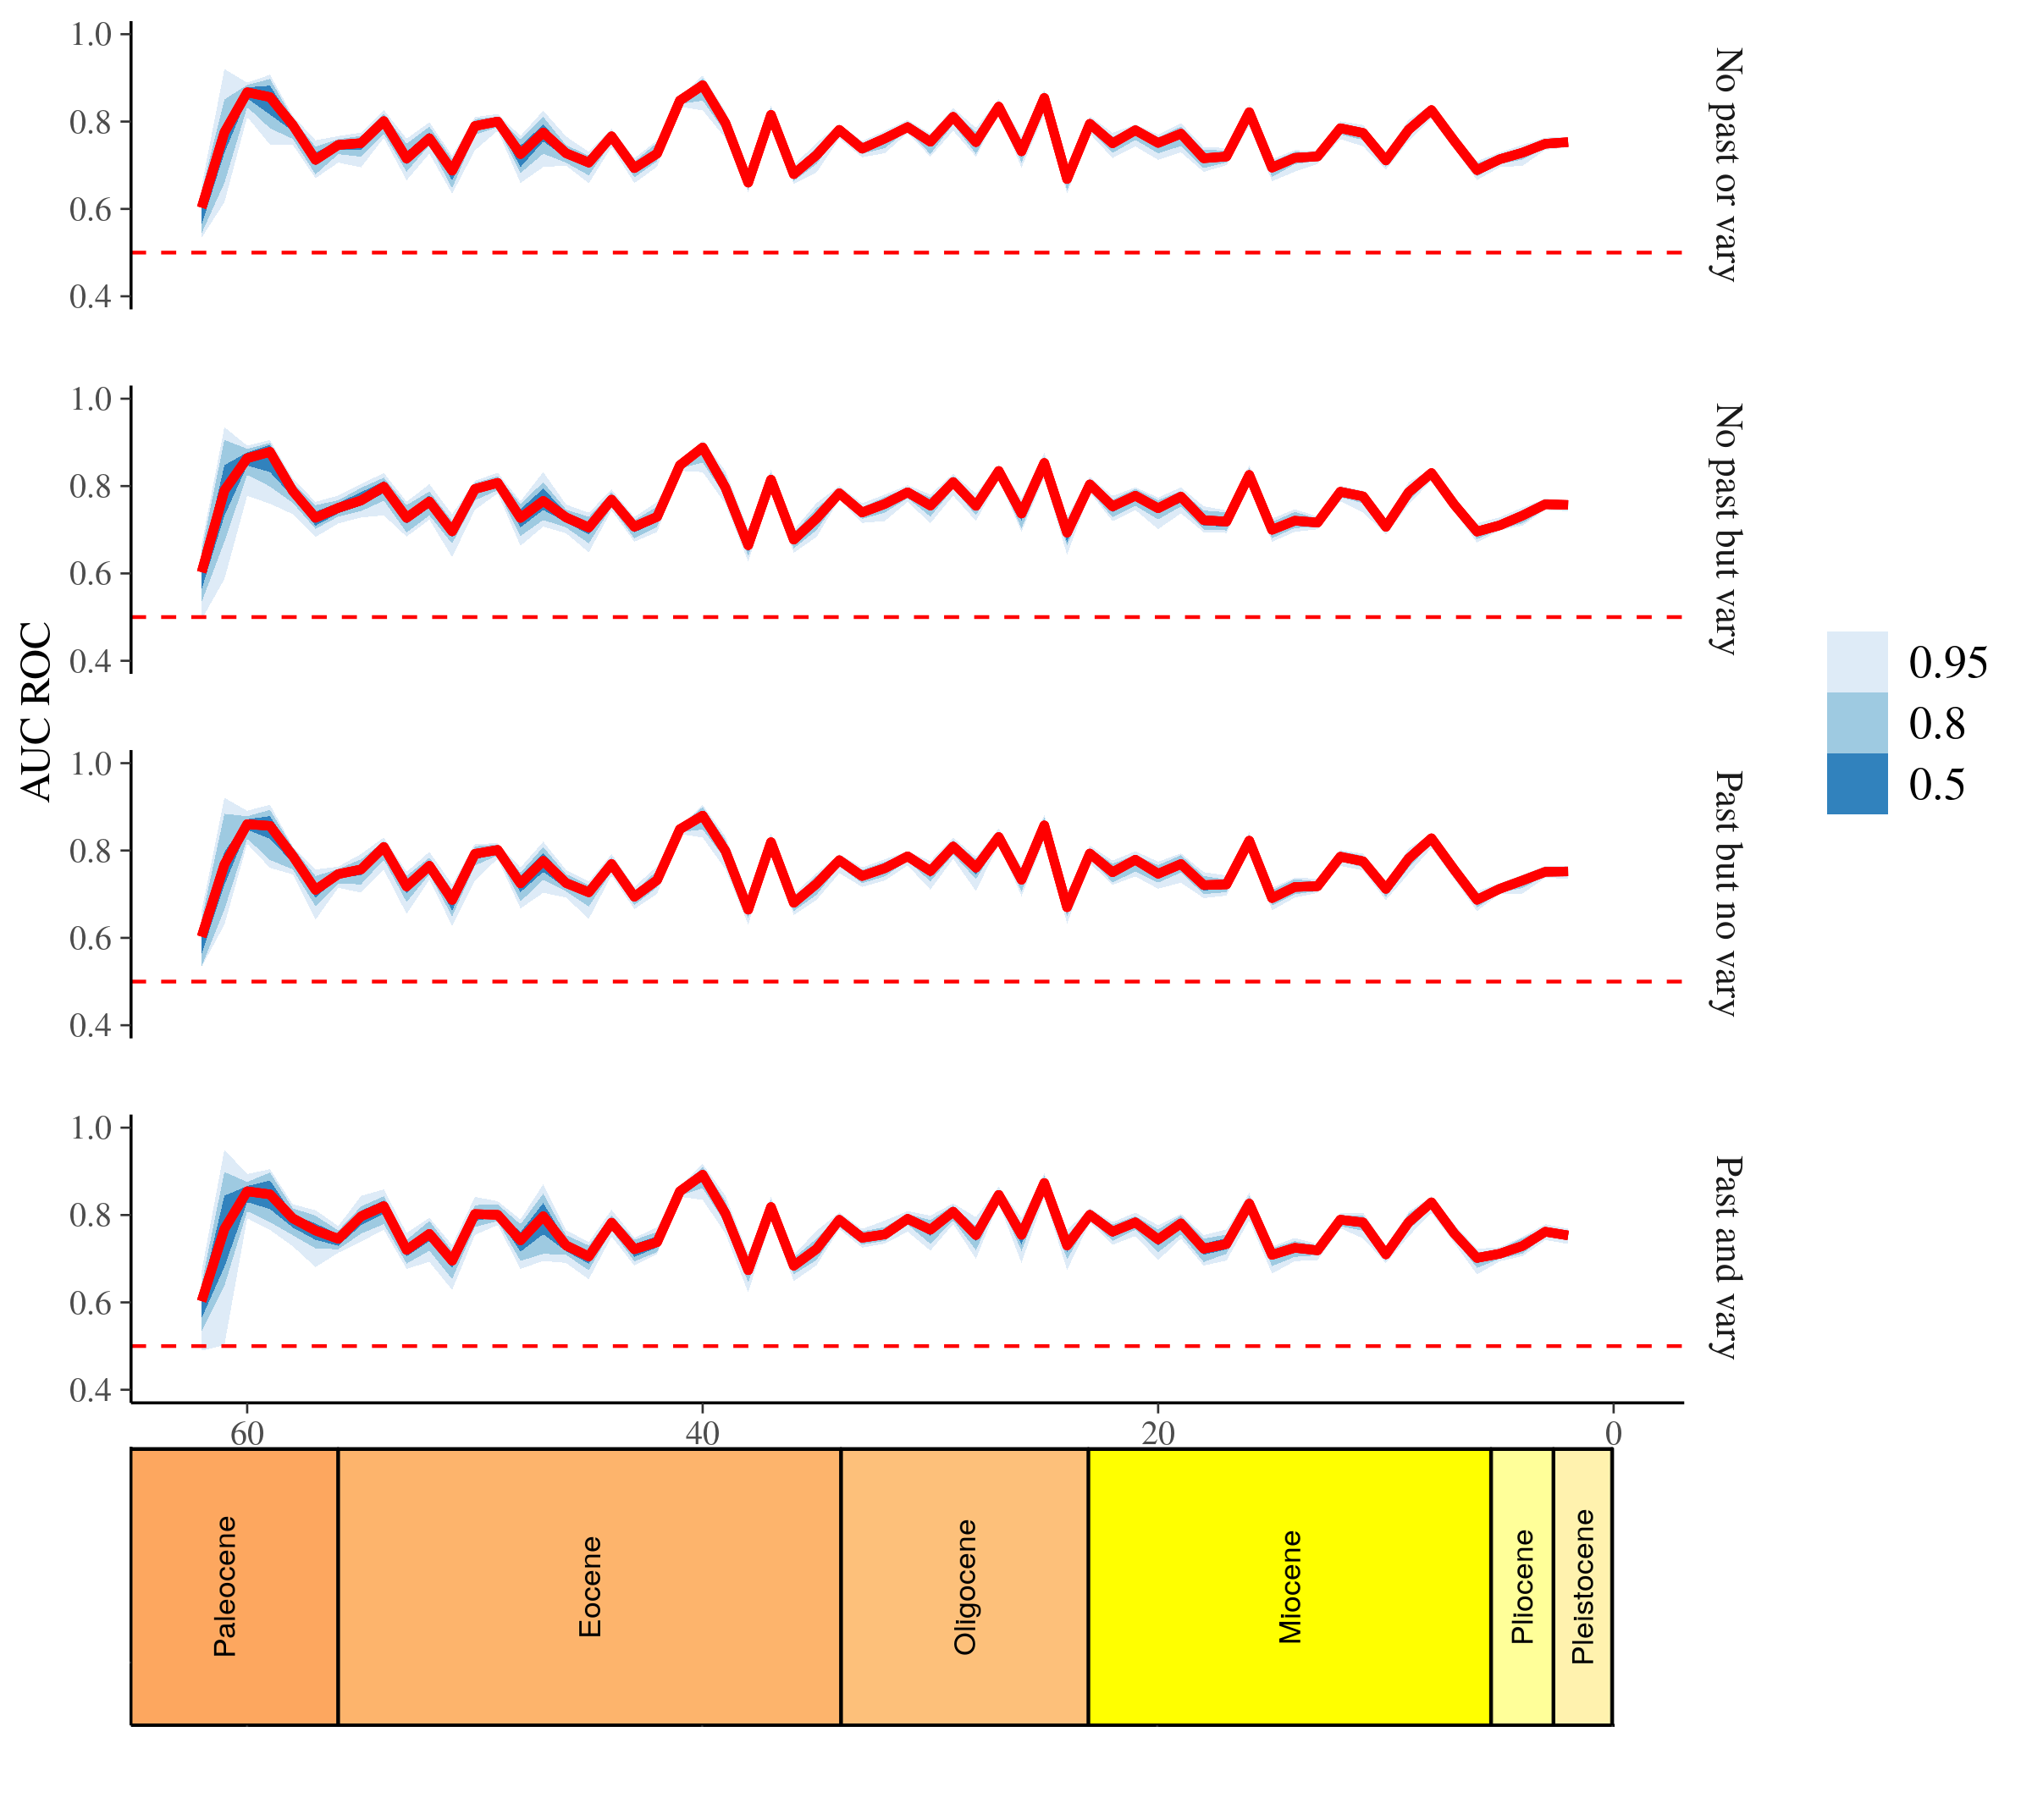
\includegraphics[width=\textwidth,height=0.5\textheight,keepaspectratio=true]{../results/figure/auc_ts}
  \caption{Comparison between the posterior predictive AUC estimates for each of the time intervals for each of the four models. These estimates are reflections of each model's fit to the various time intervals. The red line corresponds to the median AUC value, while the envelopes correspond to multiple credible intervals as indicated in the legend. In all cases, higher AUC values indicate greater predictive performance versus lower AUC values.}
  \label{fig:auc_ts}
\end{figure}


When the posterior predictive distributions of the in-sample AUC estimates are presented by taxonomic group, some heterogeneity in model adequacy is revealed (Fig. \ref{fig:auc_taxon}). While in all cases the model with the highest average in-sample AUC is the parameter-rich ``past and vary'' model, the amount of difference between the models varies by taxonomic group in ways not observable from the pooled estimates (Fig. \ref{fig:auc_hist}). For example, the difference between the ``past and vary'' model and the others is more pronouced for Calcareous nannoplankton and Dinoflagellates, and smaller for the Foraminifera and Radiolaria. 
\begin{figure}[ht]
  \centering
  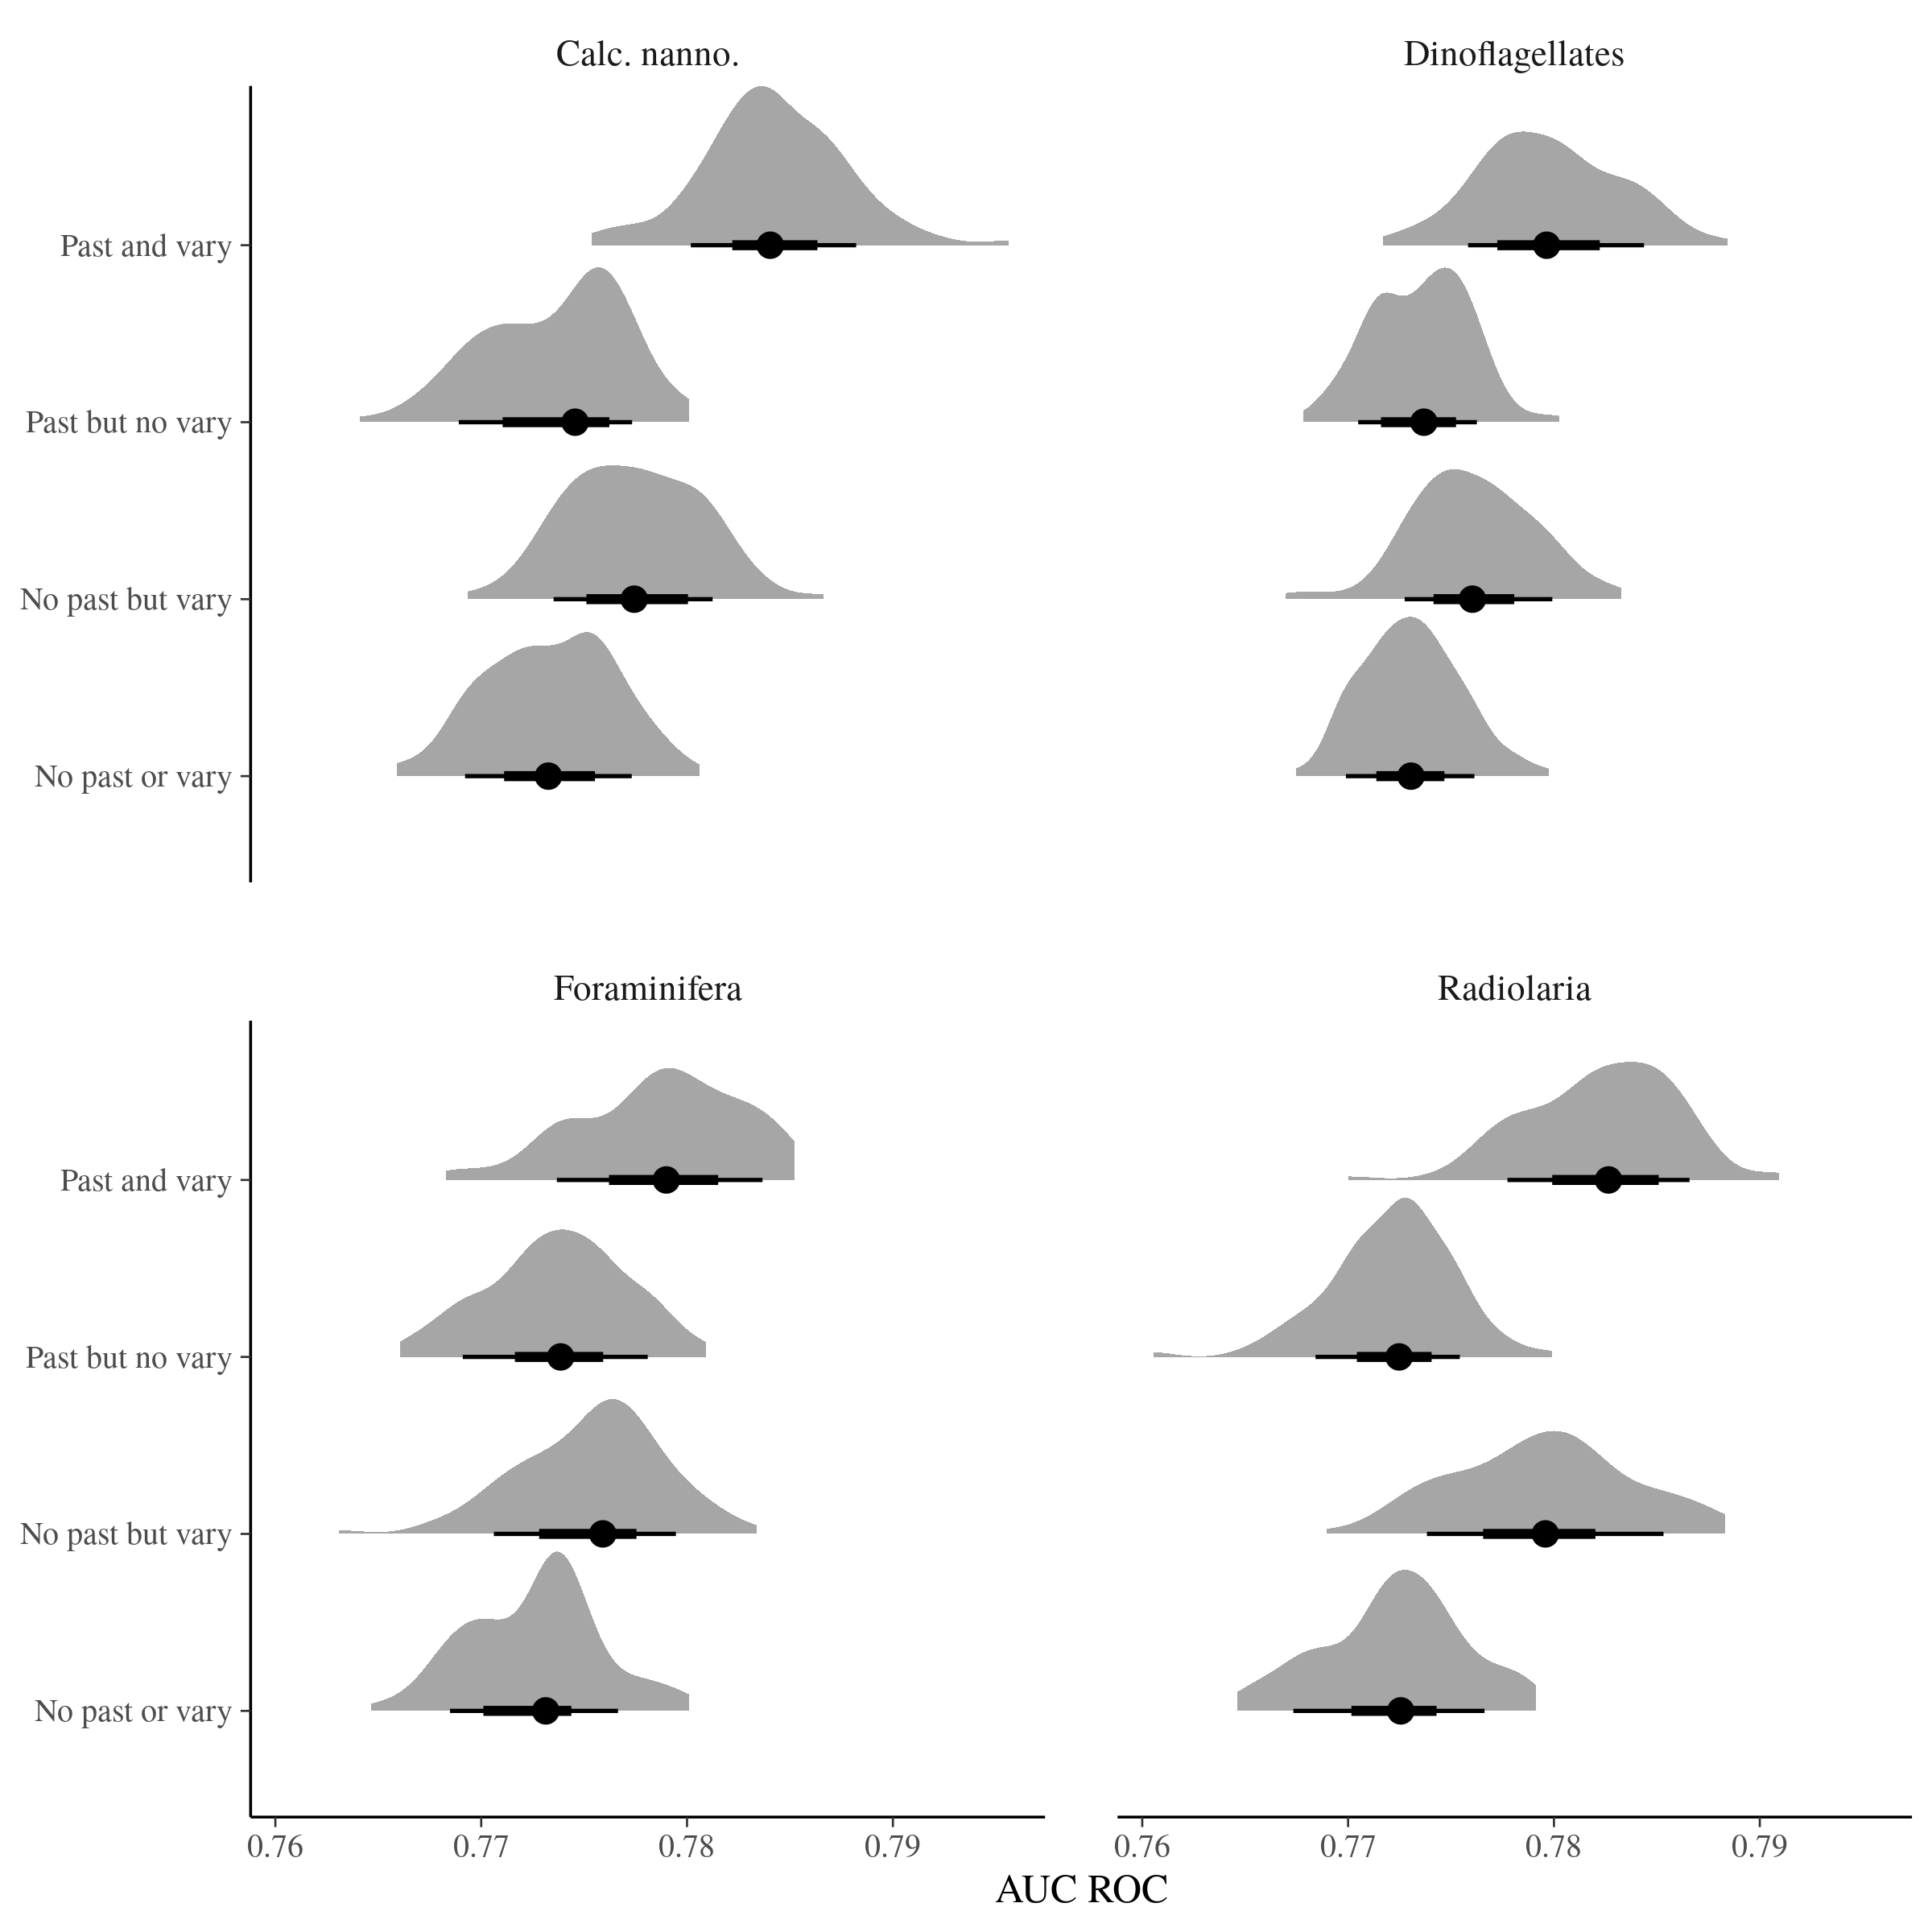
\includegraphics[width=\textwidth,height=0.5\textheight,keepaspectratio=true]{../results/figure/auc_taxon}
  \caption{Comparison of posterior predictive AUC estimates for each of the four models, arranged by taxonomic group. These estimates reflect each model's fit to the various taxonomic groups present in this analysis. The densities reflect the posterior distribution of the estimates, and below each density is marked the median AUC value along with the 50\% and 80\% credible intervals. In all cases, higher AUC values indicate greater predictive performance versus lower AUC values.}
  \label{fig:auc_taxon}
\end{figure}

Finally, when the posterior predictive distributions of the in-sample AUC estimates are presented over time and by taxonomic group, the reasons for the differences in model adequacy between the taxonomic groups becomes more apparent (Fig. \ref{fig:auc_taxon_time}), in particular the marginally better performance of the ``past and vary'' model over the other three. 

For many taxon/model combinations there are one or more time periods where posterior predictive in-sample AUC has a median value less than or equal to 0.5 -- AUC value of 0.5 indicates that the model's predictions are no better than random (Fig. \ref{fig:auc_taxon_time}). However, this pattern is absent for the posterior predictive distribution of Foraminfera and Radiolaria for the ``past and vary'' model. Additionally, these periods of low model performance are rarer for the posterior predictive distribution of the ``past and vary'' model for calcareous nannoplankton and Dinoflagellates when compared to the other three models.
\begin{figure}[ht]
  \centering
  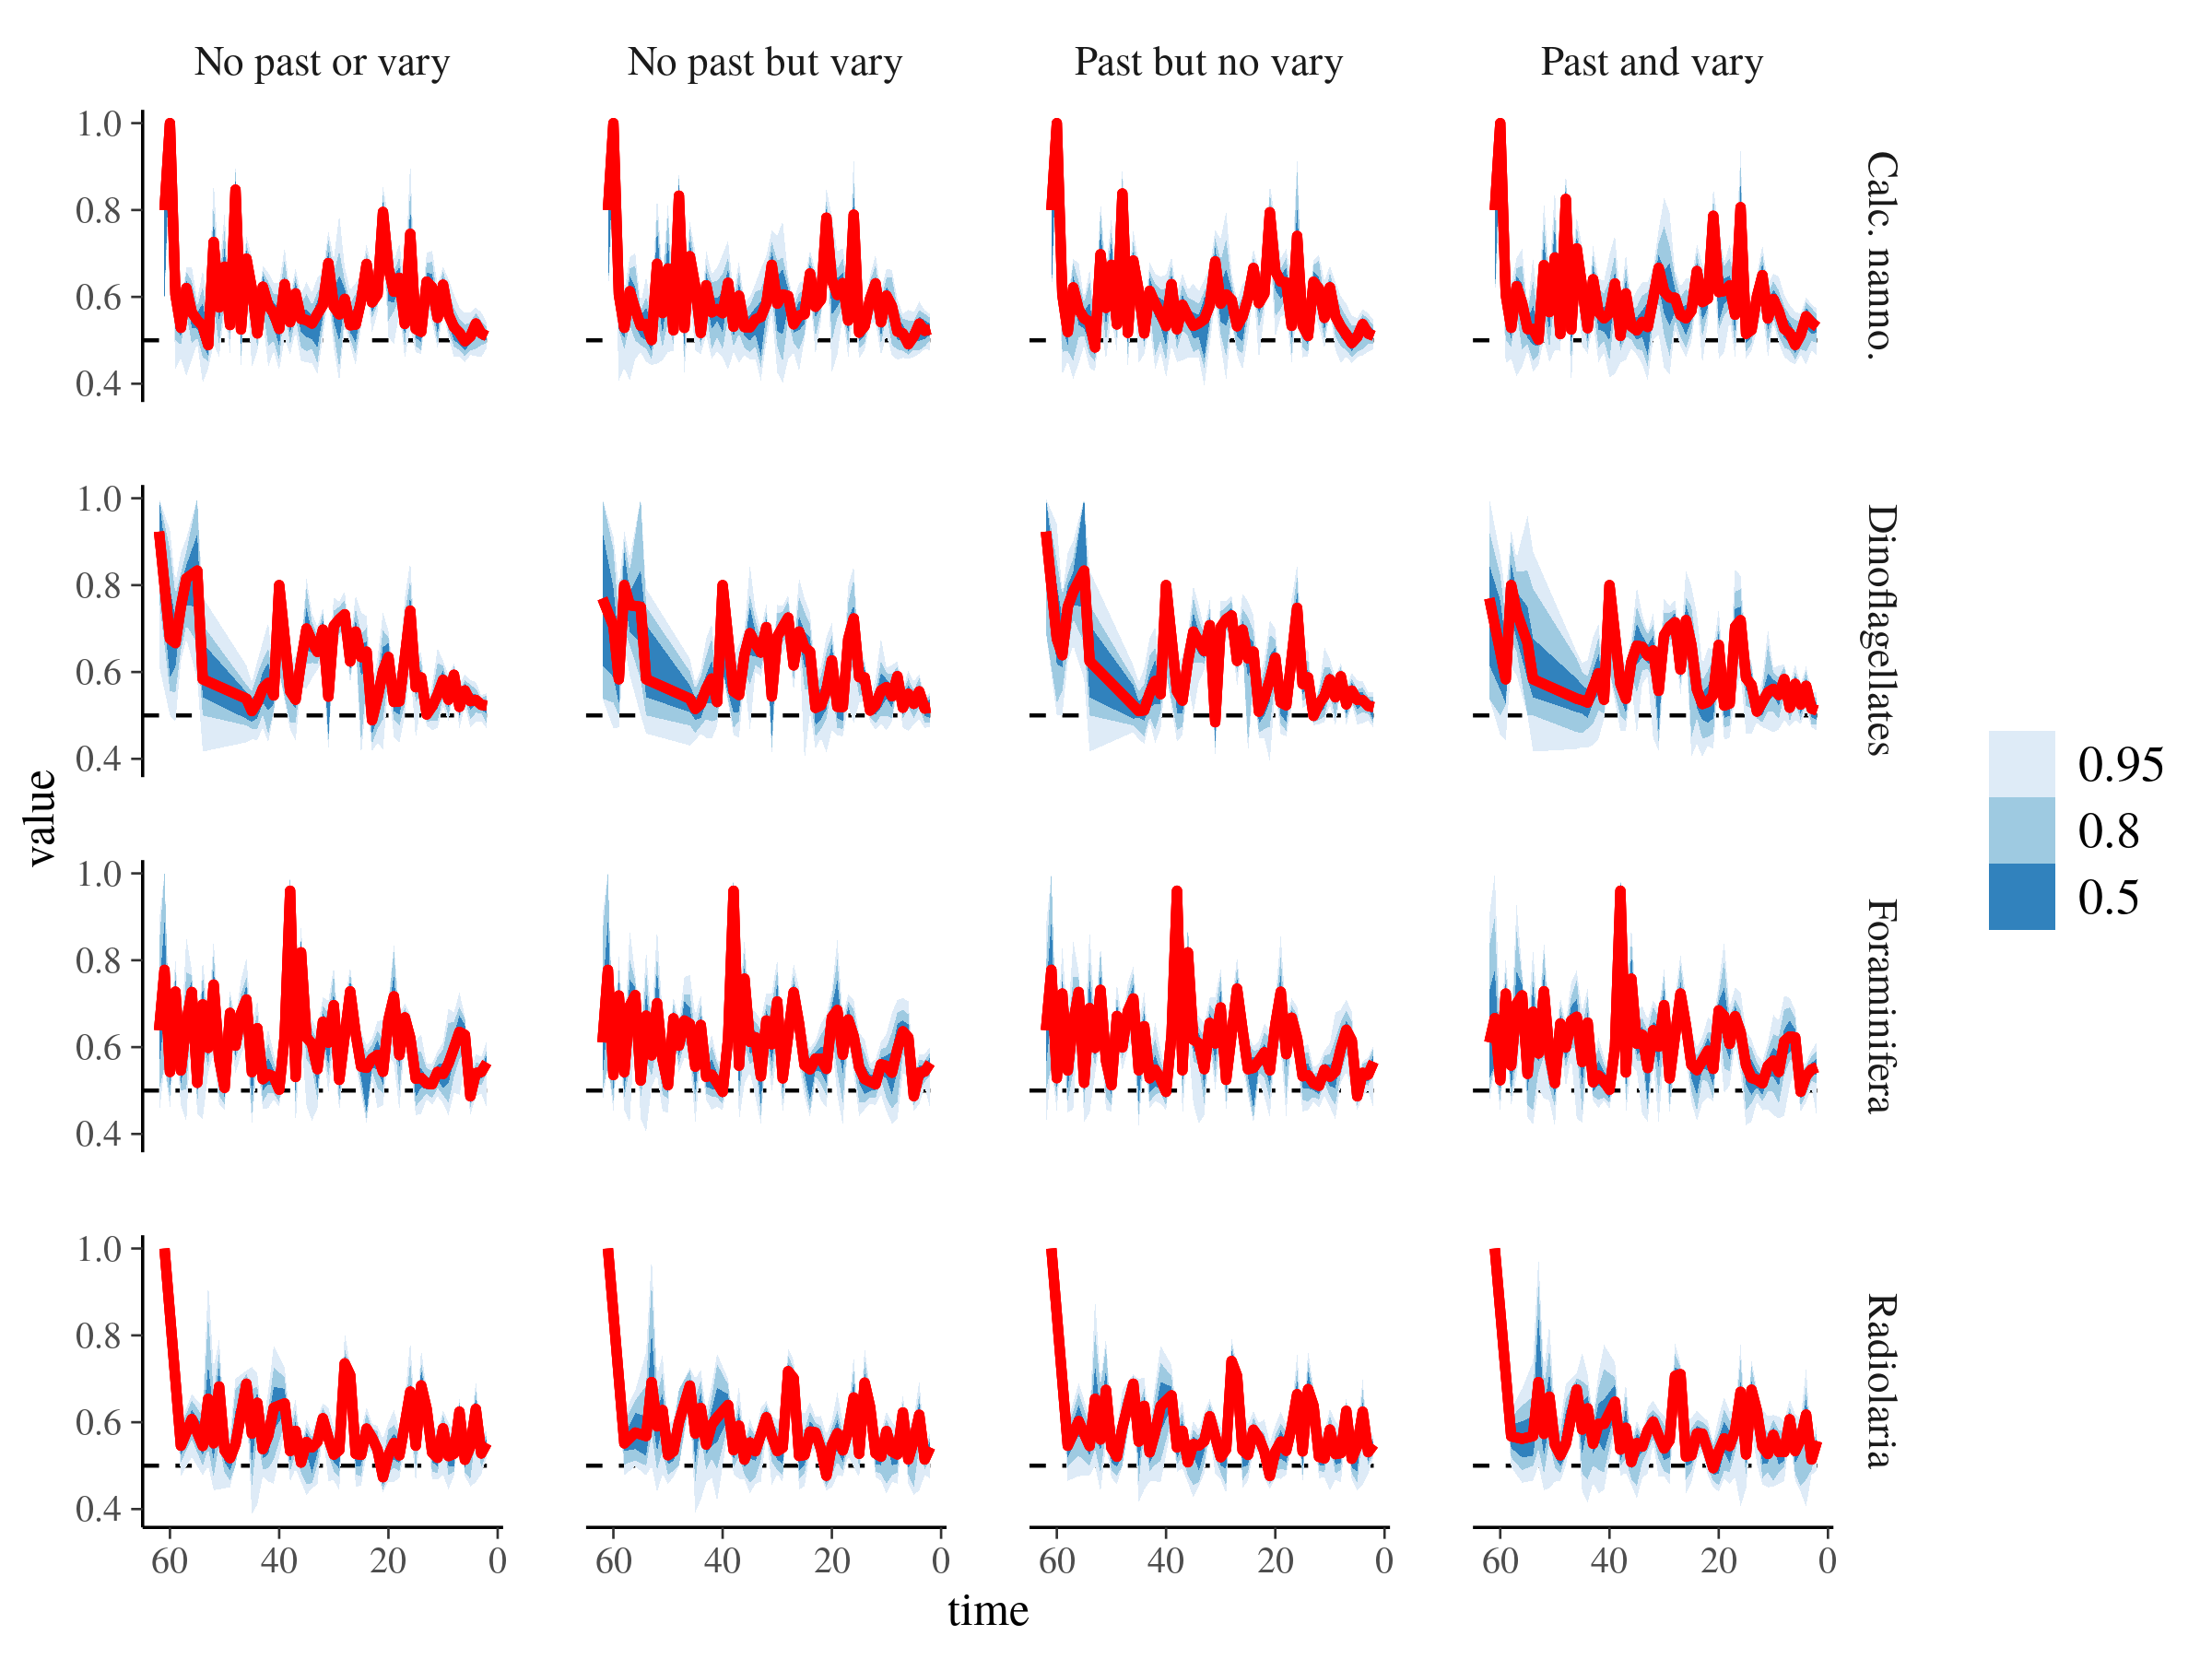
\includegraphics[width=\textwidth,height=0.5\textheight,keepaspectratio=true]{../results/figure/auc_taxon_time}
  \caption{Comparison of posterior predictive AUC estimates for each of the four models, arranged over time and by taxonomic group. These estimates reflect each model's fit to the various taxonomic groups over time. The red line corresponds to the median AUC value, while the envelopes correspond to multiple credible intervals as indicated in the legend. In all cases, higher AUC values indicate greater predictive performance versus lower AUC values.}
  \label{fig:auc_taxon_time}
\end{figure}



\section{Cross-validation}

Expected out-of-sample predictive performance was estimated using five-fold cross-validation, modified for time series data CITATION. This procedure yields four posterior (predictive) distributions, each corresponding to AUC values calculated from model-based predictions compared to the extinction state of the hold-out data. These four posterior predictive distributions are pooled to yield a posterior predictive distribution of expected out-of-sample performance -- the resulting distributions tend to be very multimodal due to their very nature being fit to and estimated from different data sets and amounts of data CITATION. Additionally, multimodality increases with model complexity (Fig. \ref{fig:fold_auc}) -- this makes sense as the more complex models allow for predictor effects to vary with time, allowing for a greater range in possible parameter values which in turn yield a greater range of posterior predictions.

Comparison between the posterior predictive distributions of expected out-of-sample AUC (Fig. \ref{fig:fold_auc}) reveals a similar range in plausible values for all models as the in-sample AUC posterior predictive distributions (Fig. \ref{fig:auc_hist}). Interestingly, the differences between the posterior predictive distributions for the models have decreased. For example, the ``past and vary'' model not clearly better than either of the ``no past or vary'' and ``past and no vary'' models (Fig. \ref{fig:fold_auc}), which were shown earlier to be obviously worse-performing models based on in-sample performance (Fig. \ref{fig:auc_hist}). These differences means that the rank order of median out-of-sample AUC is different from the rank order of median in-sample AUC. However, the shapes of the posterior distributions means interepting from the median values is incorrect -- the models are effectively indistinguishable in their expected out-of-sample AUC values.

Additionally, the quality of expected out-of-sample performance is not great, with average out-of-sample AUC for each of our models estimated to be between 0.7 and 0.8 which is far from perfect. This result means that we would expect to correctly rank two species in order of most to least likely to go extinct 70-80\% of the time. However, this expected out-of-sample performance is approximately the same as the in-sample performance results (Fig. \ref{fig:auc_hist}), indicating that our models would yield consistent results when generalized to future extinctions.
\begin{figure}[ht]
  \centering
  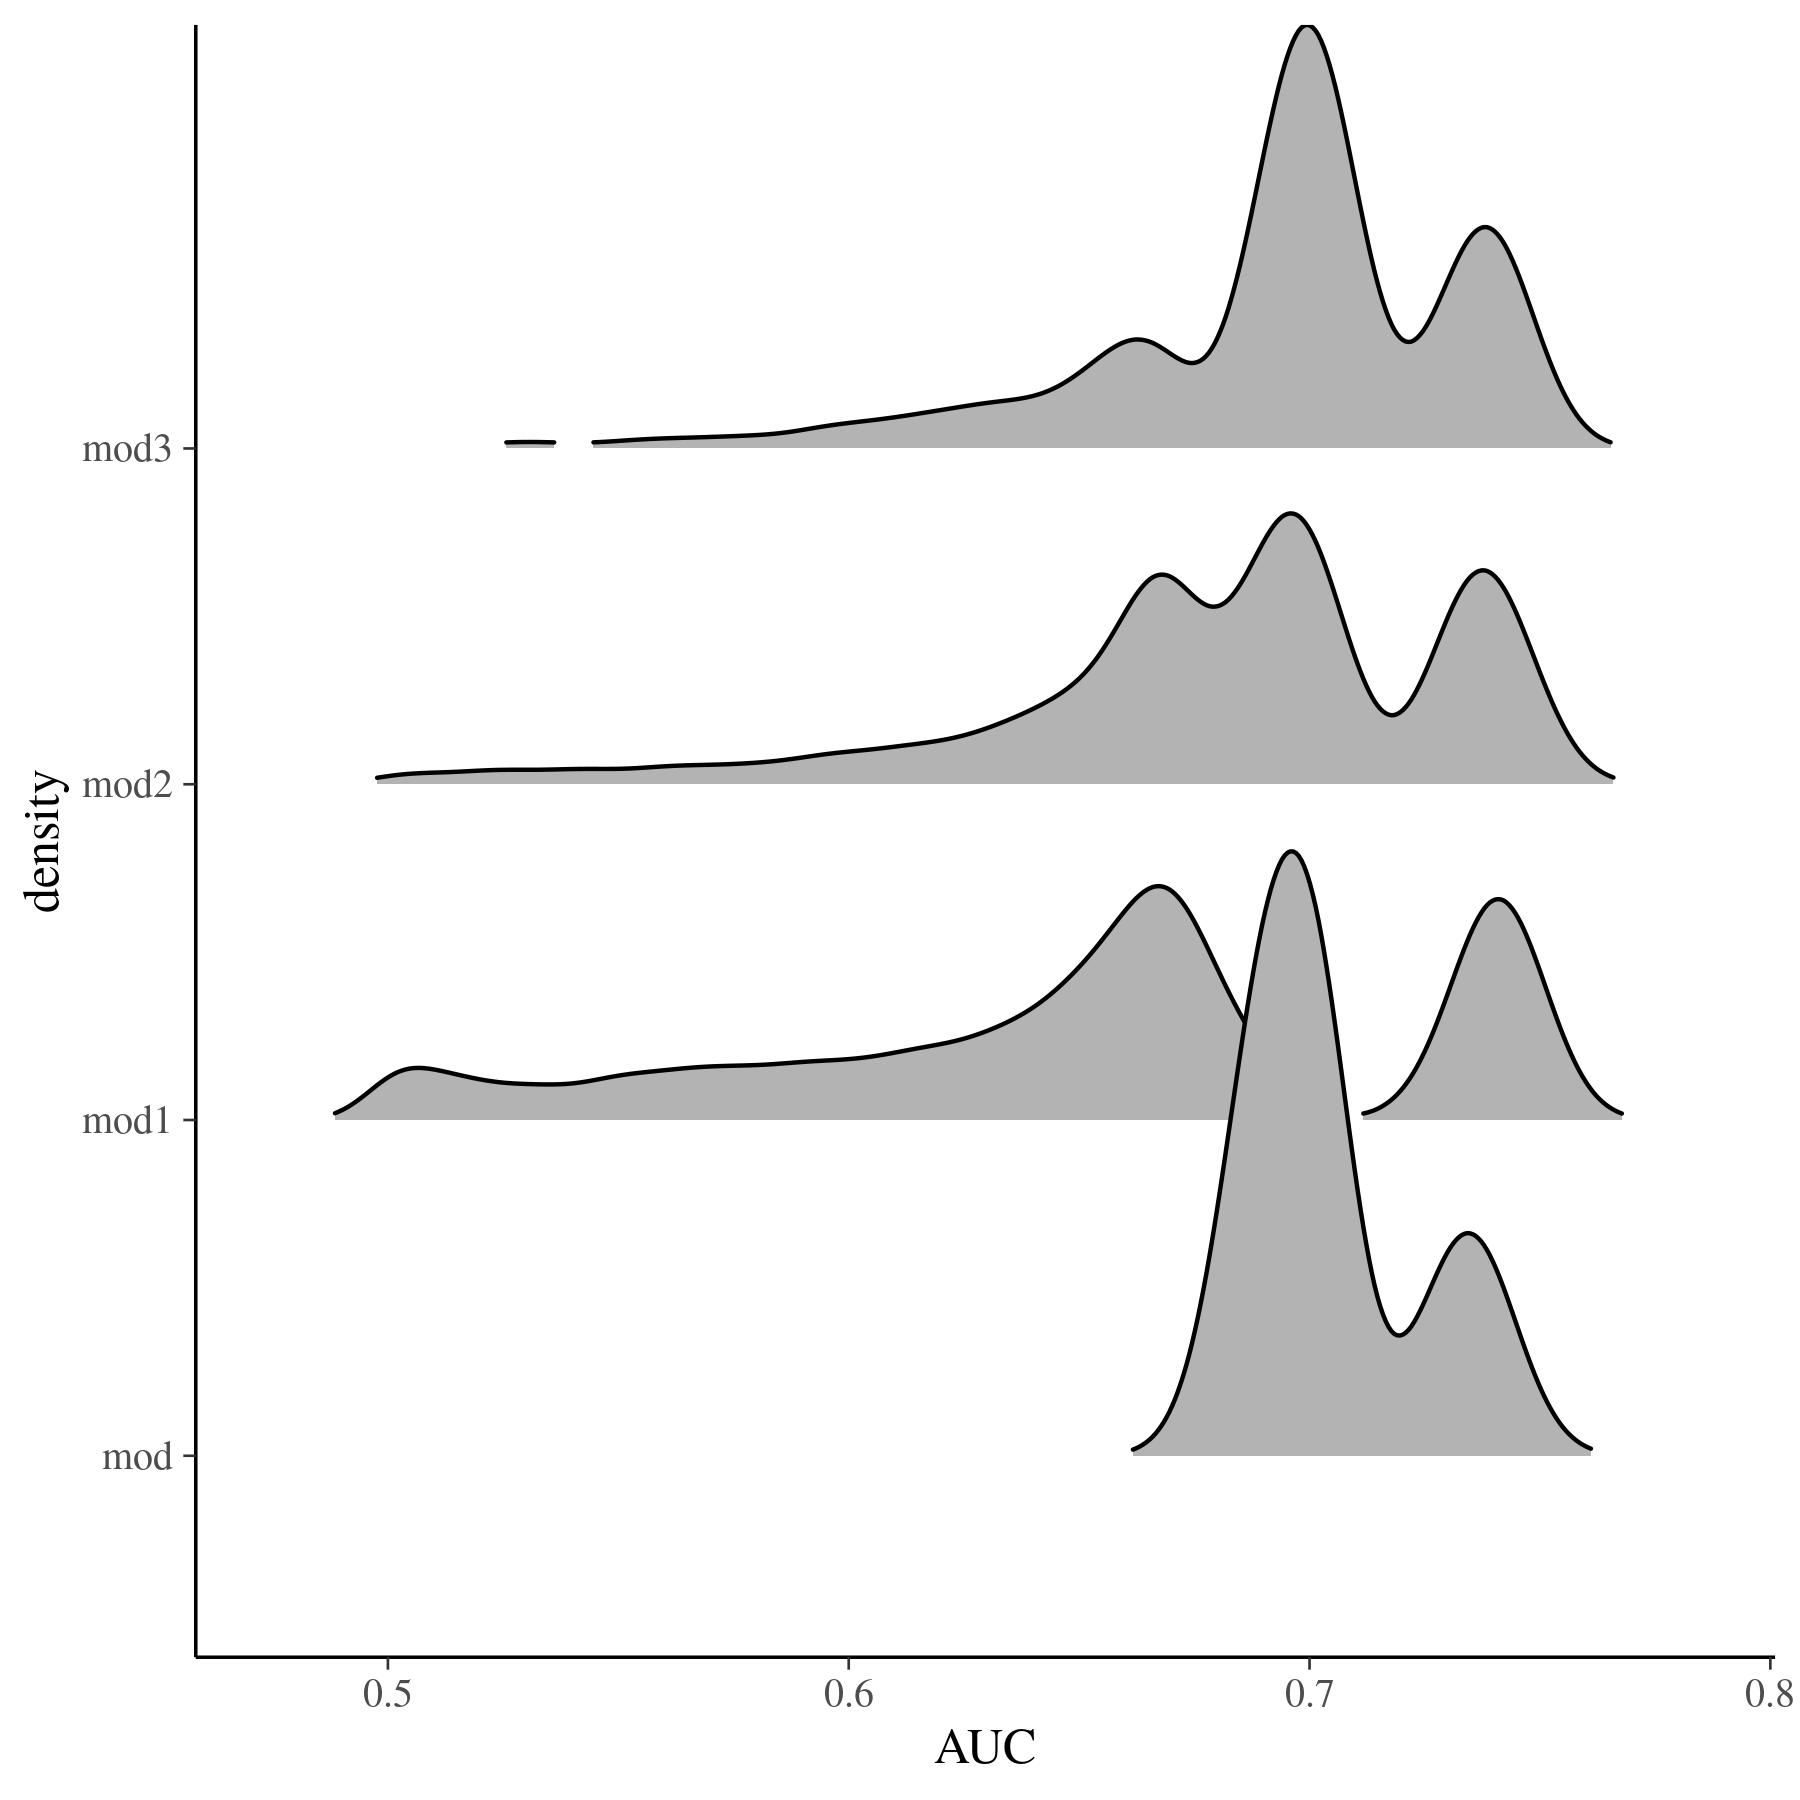
\includegraphics[width=\textwidth,height=0.5\textheight,keepaspectratio=true]{../results/figure/fold_auc}
  \caption{Results from our five-fold cross-validation of the time-series. Each labeled distribution of AUC values correspond to expected out-of-sample performance as estimated from that fold. Each fold represents a section of data being predicted from a model fit to all data before the start of that fold. Given that there are only five folds, performance is measured from predictions for four of the folds.}
  \label{fig:fold_auc}
\end{figure}

When the posterior predictive distribution of expected out-of-sample AUC is presented as a time series, the similarity between the models is even more apparent (Fig. \ref{fig:fold_auc_time}). While the width of the credible intervals at various time points varies between the models, the overall picture of expected out-of-sample AUC is almost identical when you compare the models -- periods of relatively better or worse performance map identically between the time series.
\begin{figure}[ht]
  \centering
  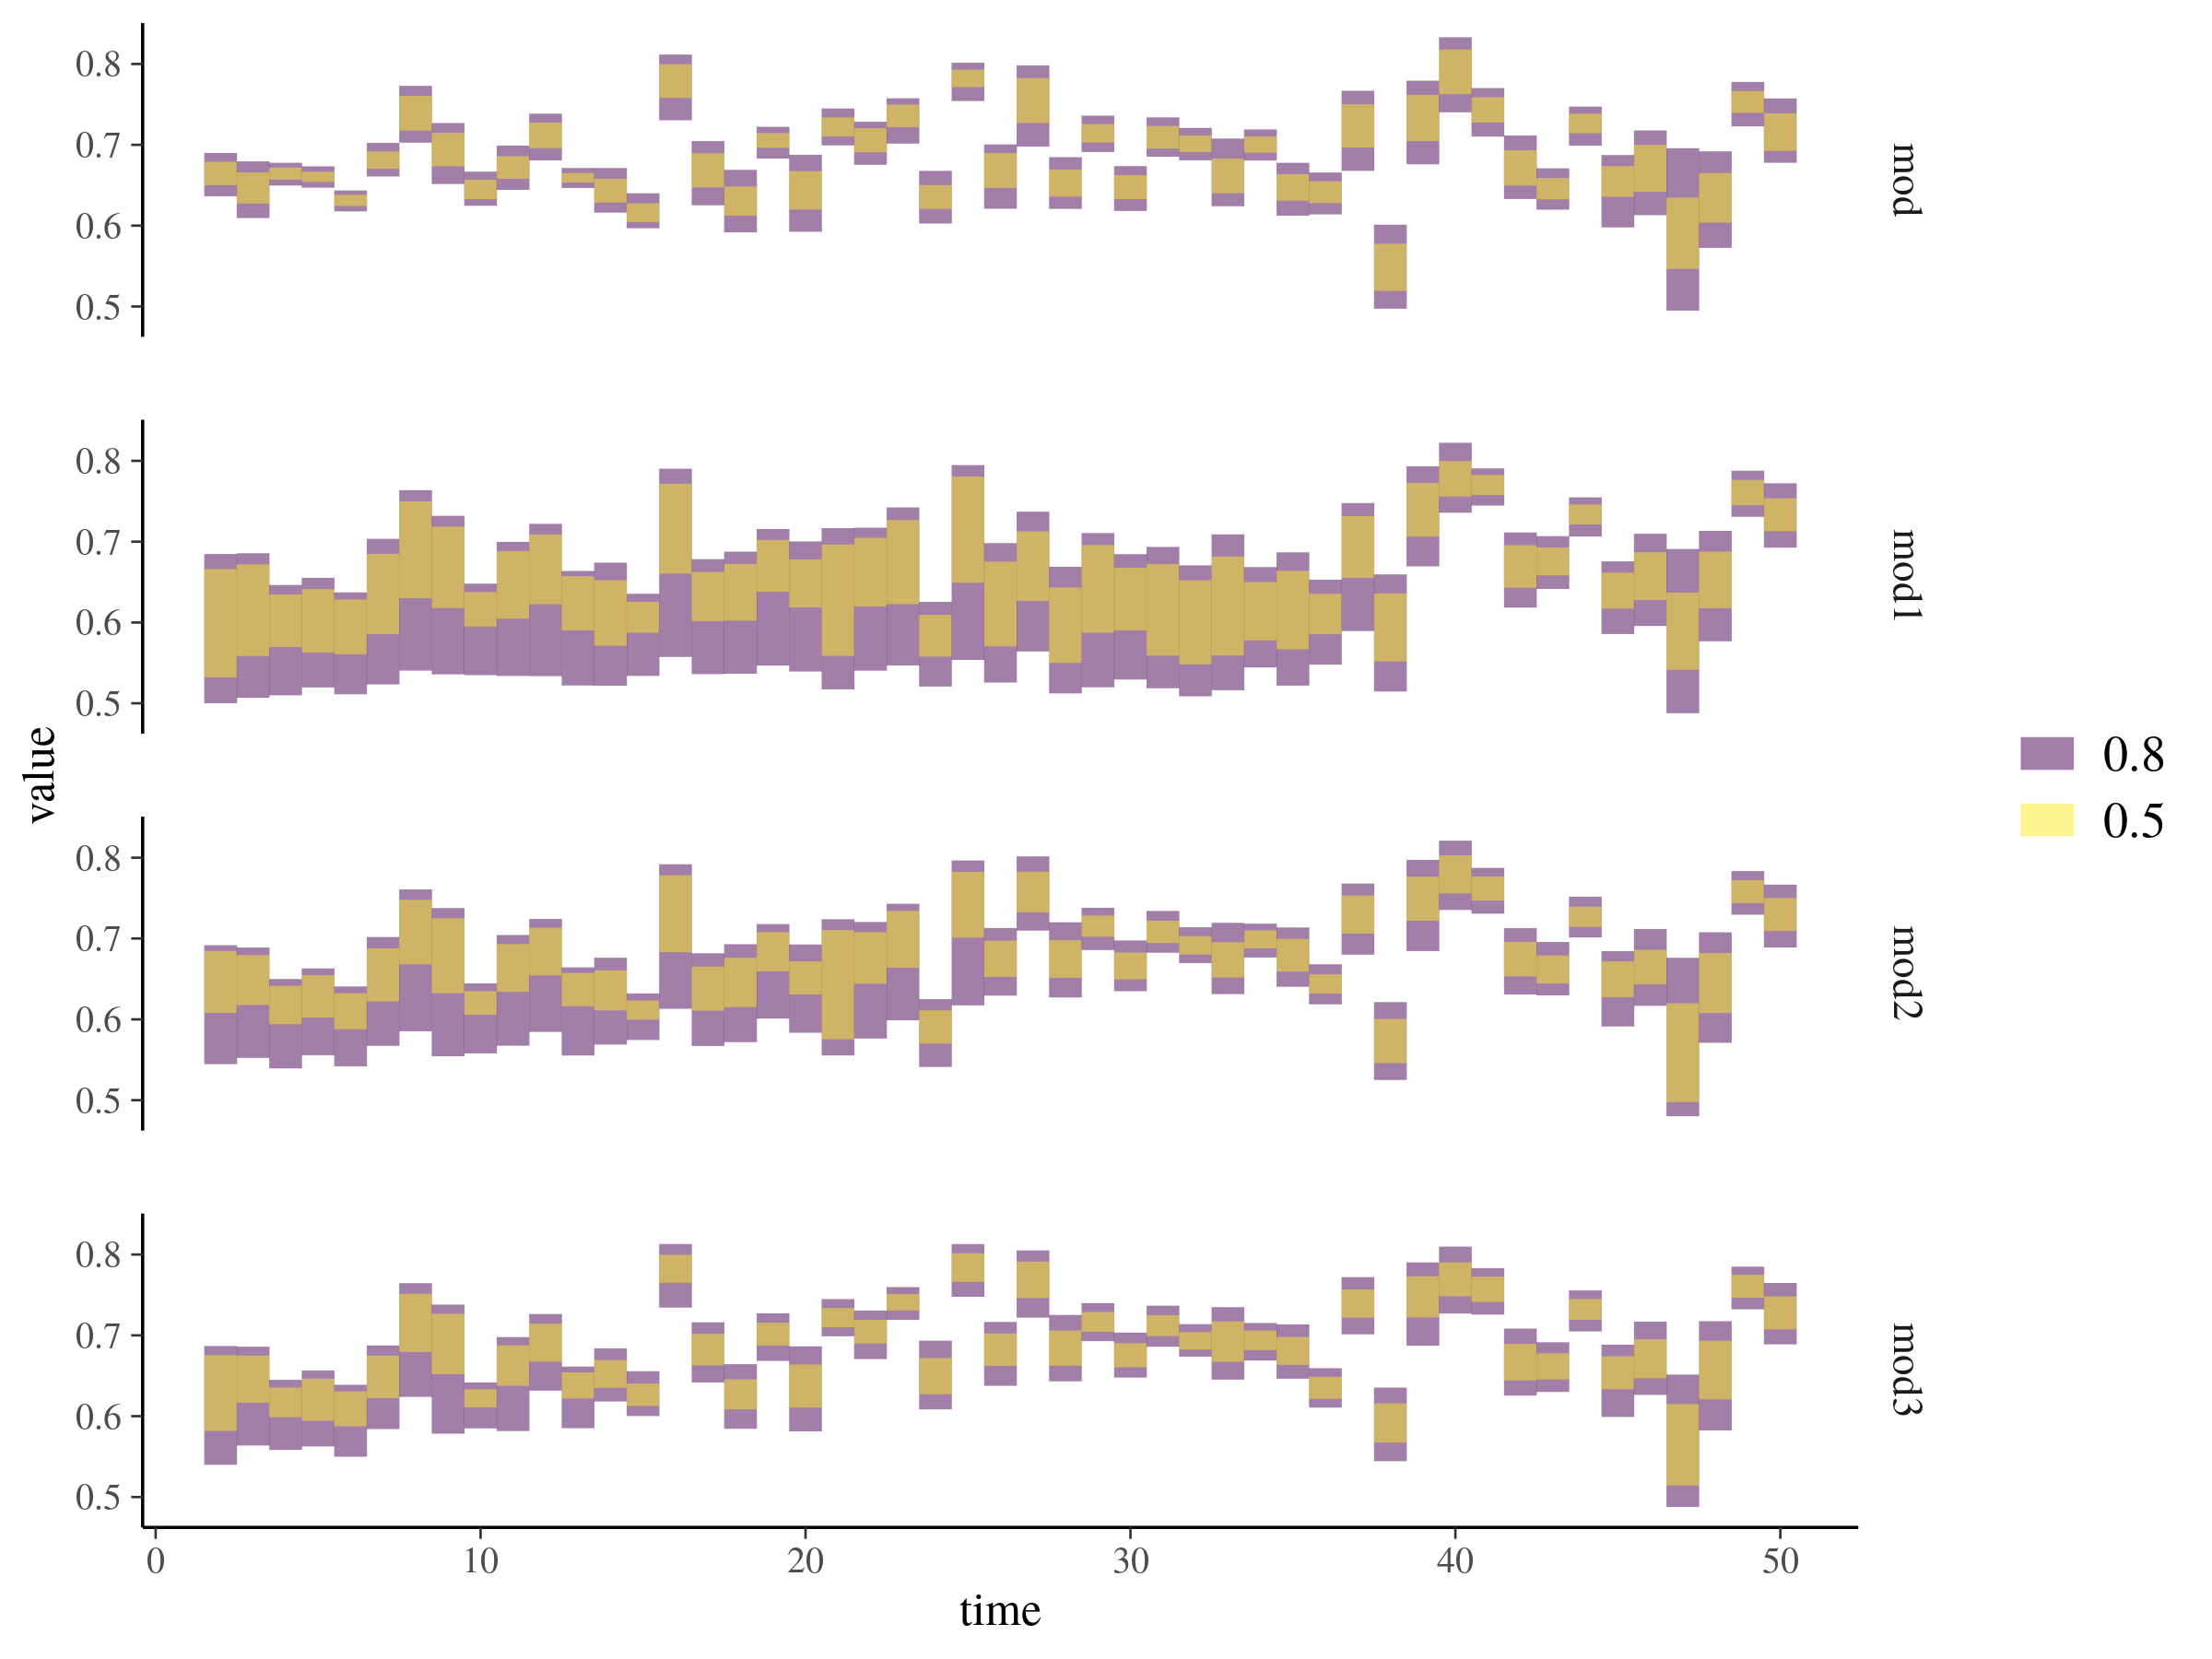
\includegraphics[width=\textwidth,height=0.5\textheight,keepaspectratio=true]{../results/figure/fold_auc_time}
  \caption{Comparison of out-of-sample AUC values calculated for each of the My intervals for each of the four models. The AUC of the individual My intervals within each fold is plotted to highlight the heterogentity in performance within and between folds. This presentation decomposes each of the 12-million year folds (Fig. \ref{fig:fold_auc}) into the predictions made for each of the million-year intervals. The red line corresponds to the median AUC estimate, with the envelopes corresponding to multiple credible intervals as indicated in the legend.}
  \label{fig:fold_auc_time}
\end{figure}

We can also compare expected out-of-sample AUC by taxonomic group for each of the models (Fig. \ref{fig:fold_auc_taxon}). These comparisons reveal a lot about the differences in predictive potential of the taxonomic groups. For example, the posterior predictive distributions of out-of-sample AUC for Foraminifera from all four models are approximately identical. In contrast, expected out-of-sample AUC for Radiolaria exhibits the same or similar pattern in relative model performance to the pooled comparisons (Fig. \ref{fig:fold_auc}). Additionally, we can state that our out-of-sample predictions for calcareous nannoplankton and dinoflagellates are not necessarily as precise as our estimates for Foraminifera or even Radiolaria. These results indicate that out-of-sample predictions may be easier for some taxonomic groups than others (e.g. Foraminifera versus Dinoflagellates.
\begin{figure}[ht]
  \centering
  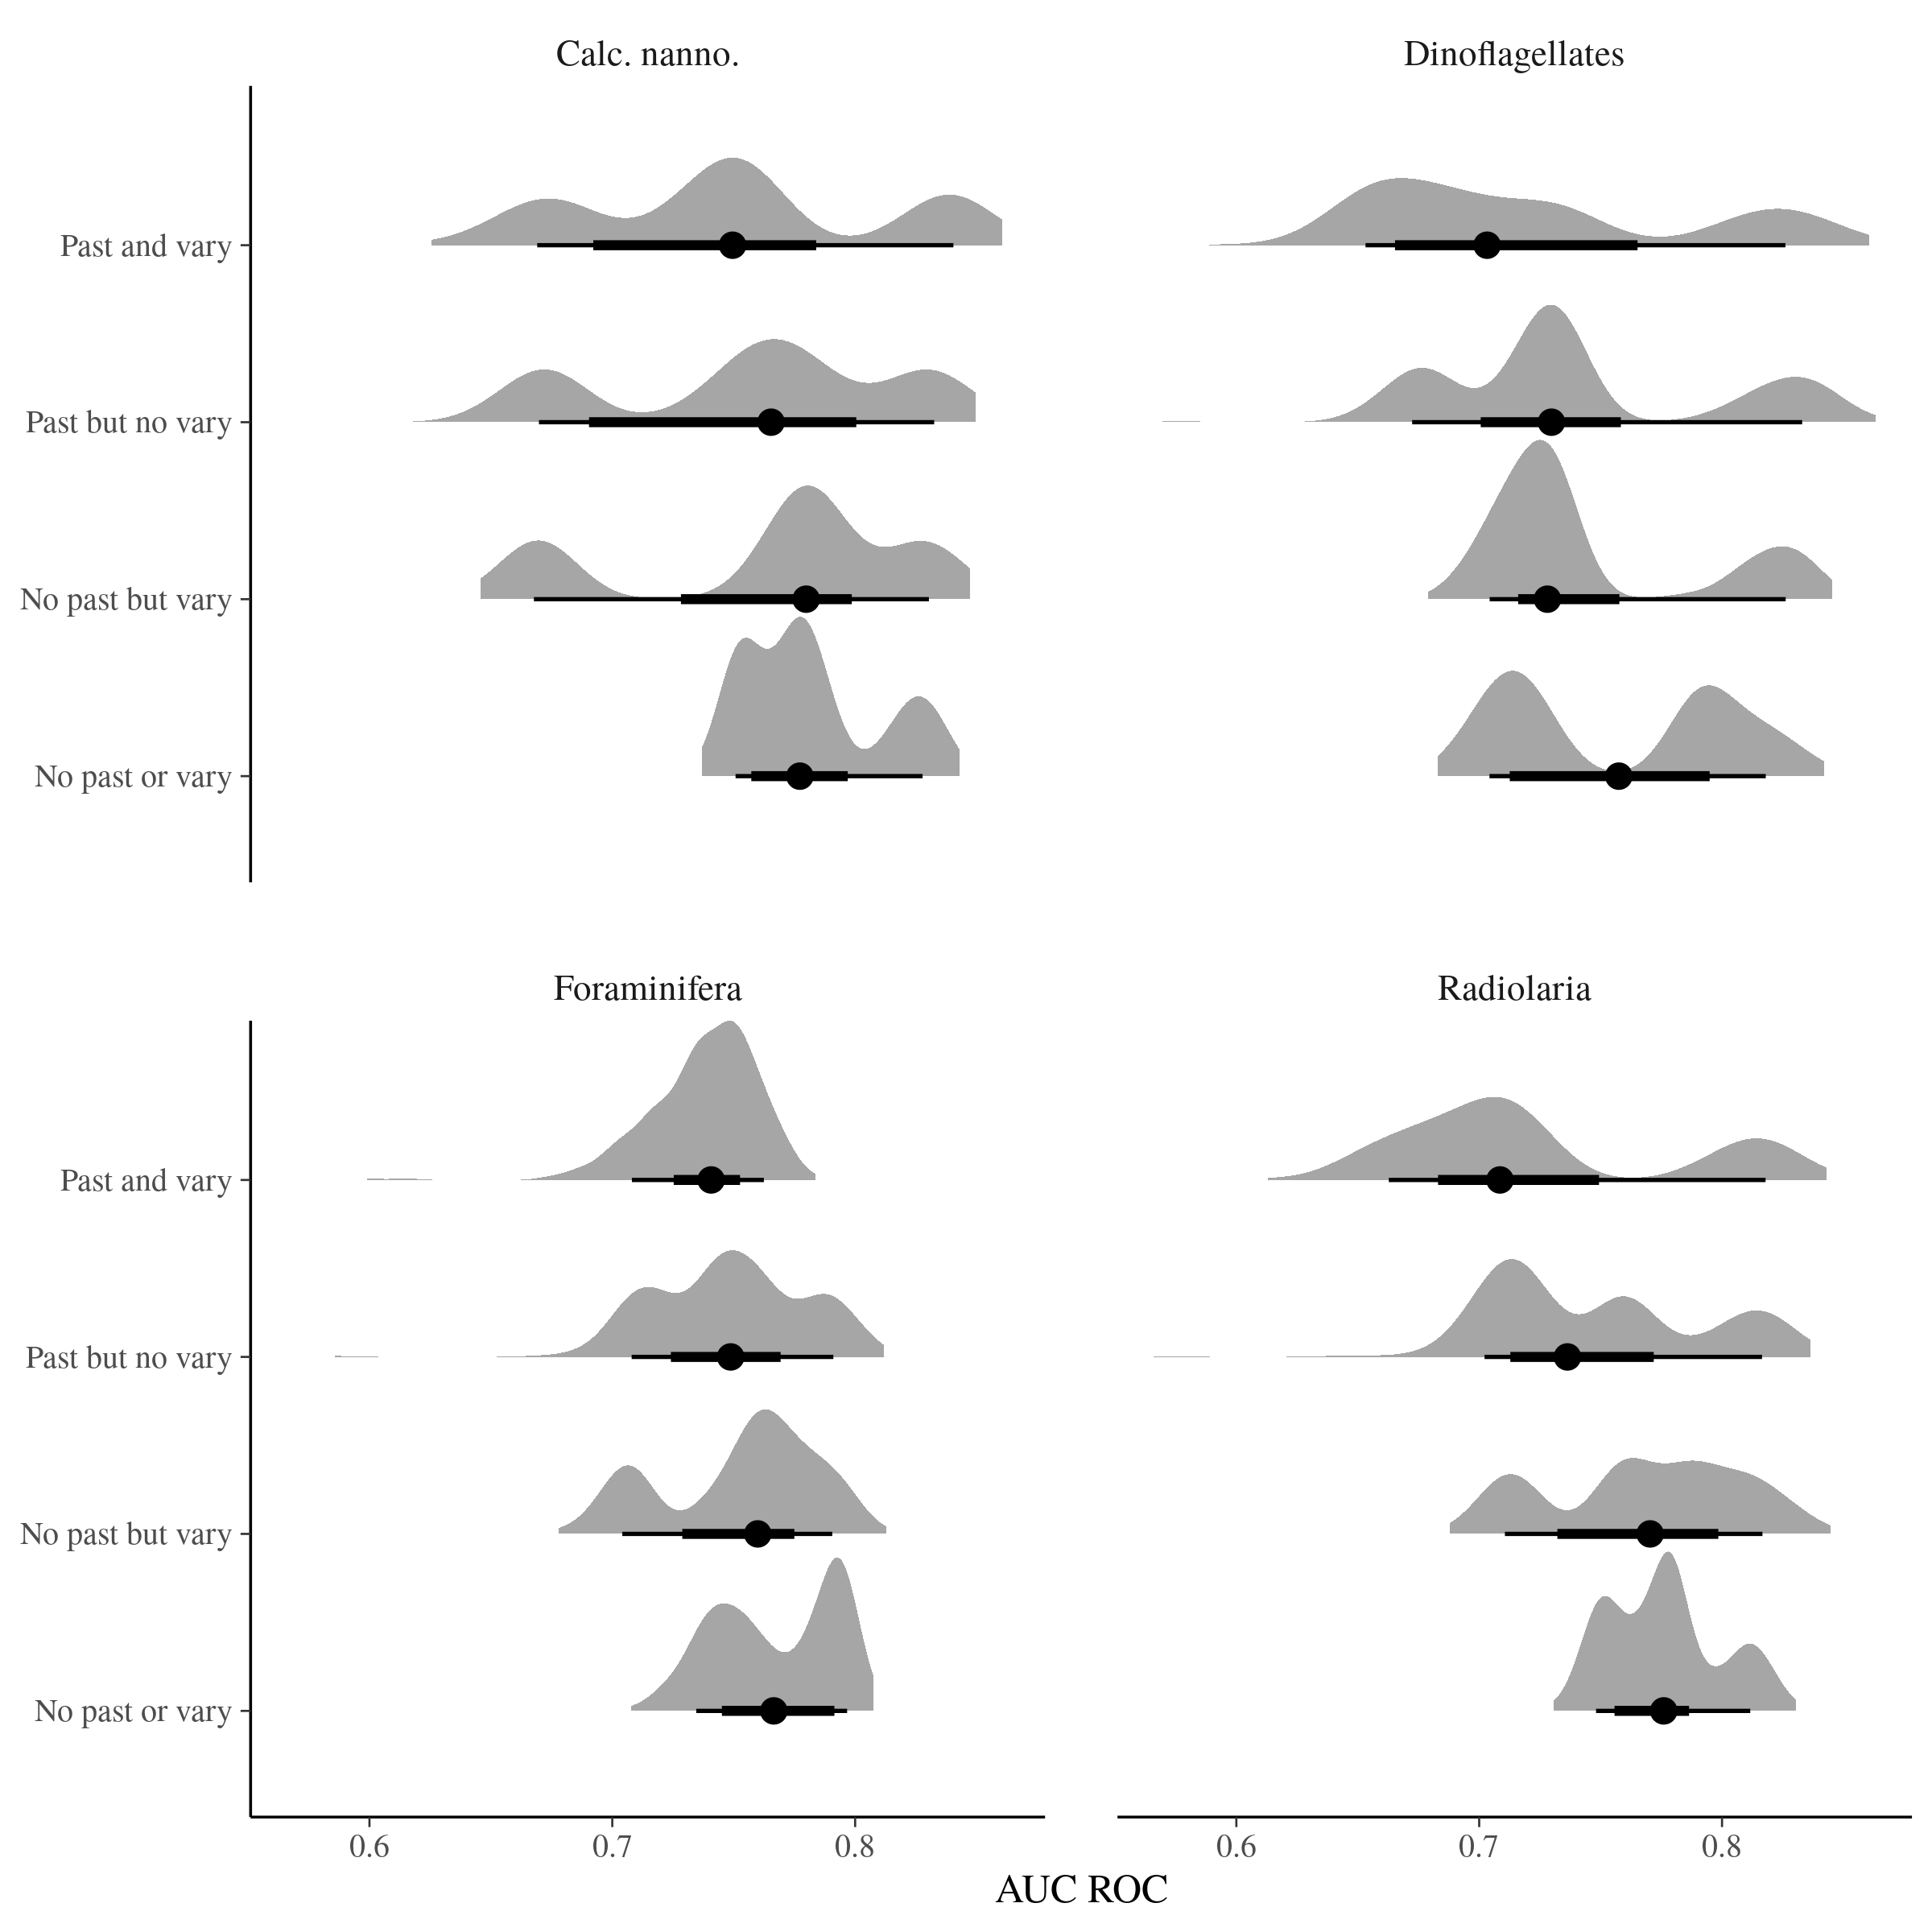
\includegraphics[width=\textwidth,height=0.5\textheight,keepaspectratio=true]{../results/figure/fold_auc_taxon}
  \caption{Comparison of out-of-sample AUC values aggregated by taxonomic group for each of the four models. Depicted for each taxon-model combination is an aggregate density of all posterior predictive estimates for each of four folds -- cross-validation estimates are commonly multi-modal as each fold presents its own challenges for prediction. Beneath these densities is marked the median estimate along with 50\% and 80\% credible intervals.}
  \label{fig:fold_auc_taxon}
\end{figure}


Finally, we can present the posterior predictive distribution of expected out-of-sample AUC over time and taxonomic group for each of the four models (Fig. \ref{fig:fold_auc_taxon_time}). For each taxonomic group, the time-series of posterior predictive values for each model are broadly congruent. 

In the analysis of the posterior predictive distributions of the in-sample AUC values for the four models, we noted that there were time intervals where the models' predictions were no better than random (Fig. \ref{fig:auc_taxon_time}). This occurrence is generally much rarer for the posterior predictive distribution of out-of-sample AUC values -- the major exception to this is Dinoflagellates, which for all four models has at least one time interval where the median the AUC of out-of-sample data were no better random. In contrast, the only other group for which median posterior predictive estimate of out-of-sample AUC reaches 0.5 is calcareous nannoplankton, and then only with the ``no past or vary'' model.
\begin{figure}[ht]
  \centering
  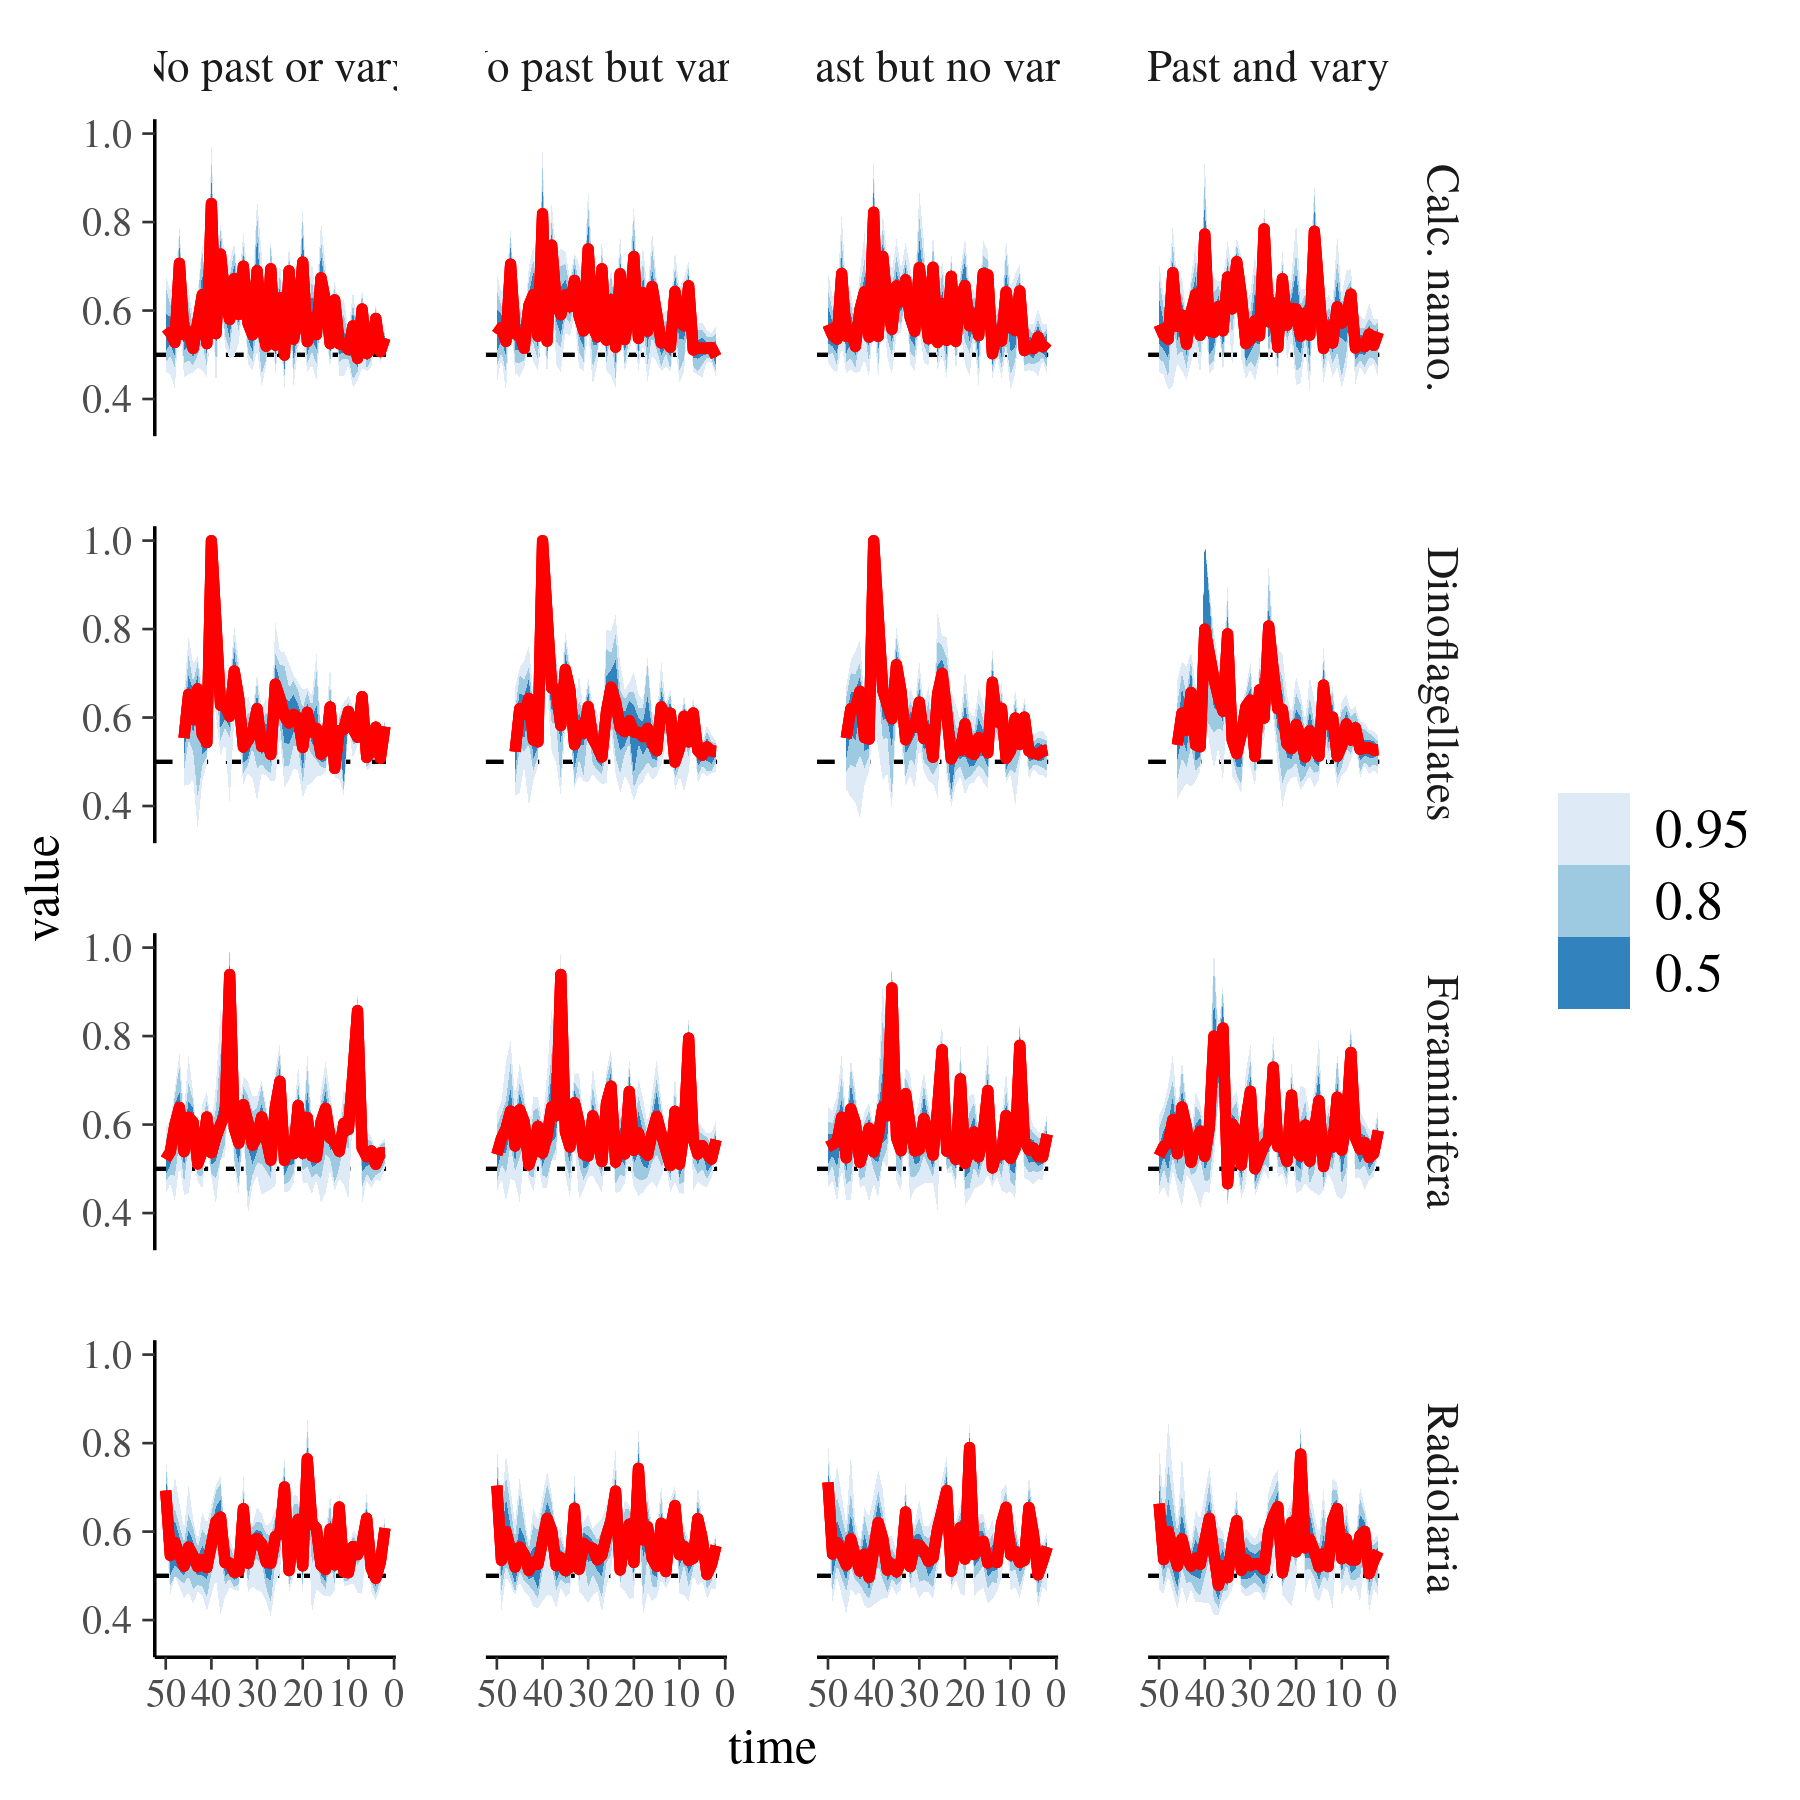
\includegraphics[width=\textwidth,height=0.5\textheight,keepaspectratio=true]{../results/figure/fold_auc_taxon_time}
  \caption{Comparison of out-of-sample AUC values over time as aggregated by taxonomic group for each of the four models. The AUC of the individual My intervals within each fold is plotted to highlight the heterogentity in performance within and between folds. This presentation decomposes each of the 12-million year folds by each of the taxonomic groups (Fig. \ref{fig:fold_auc_taxon}) into the predictions made for each of the million-year intervals. The red line corresponds to the median AUC estimate, with the envelopes corresponding to multiple credible intervals as indicated in the legend.}
  \label{fig:fold_auc_taxon_time}
\end{figure}



%\section{Parameter estimates}
%
%As expected, a species with greater than average geographic range is expected to have a greater probability of surviving than a species with average or less than average geographic range (Fig. \ref{fig:effect_est})
%
%We estimated an overall positive effect of the change in geographic range on extinction probability; this means that a species gaining in geographic range between that observation and their previous observed geographic range is associated with a greater extinction risk than a species which decreased in geographic range (Fig. \ref{fig:effect_est}). This sign of this result is consistent with virtually all previous analyses of the relation between geographic range and extinction.
%
%We estimated an overall positive effect of both global temperature and the lag of global temperature with species extinction probability (Fig. \ref{fig:effect_est}. This type of effect means that when global temperature is above the Cenozoic average, we would expect higher than average extinction risk. Similarly, if global temperature was above the Cenozoic average in the time interval before the current one, we would also expect higher than average extinction risk. This means that during a run of above Cenozoic average global temperatures (2+ intervals) we would expect an even greater extinction risk than if just the current interval is of above average temperature. These results imply that, on average, the species during Paleogene had a greater extinction probability that species during the Neogene.
%
%% effects, average
%\begin{figure}[ht]
%  \centering
%  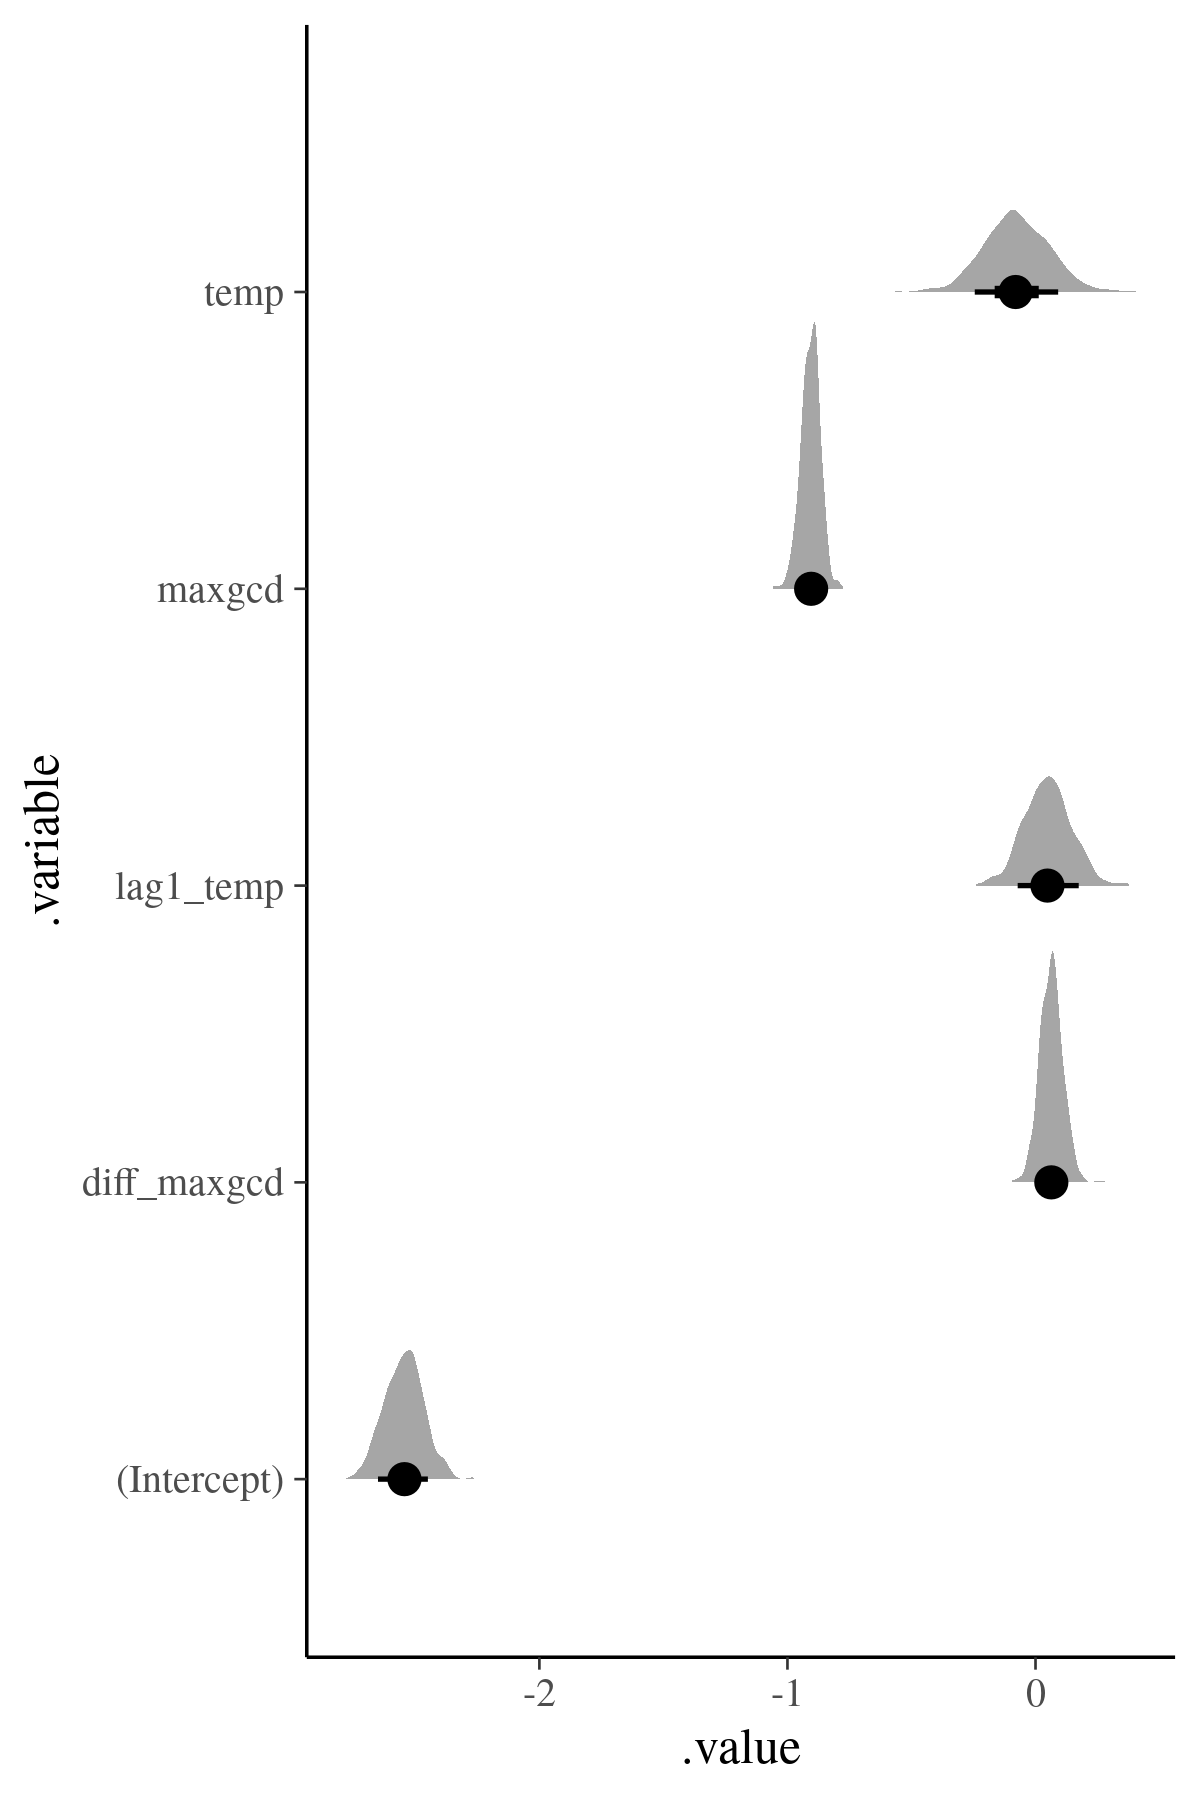
\includegraphics[width=\textwidth,height=0.5\textheight,keepaspectratio=true]{../results/figure/effect_est}
%  \caption{Posterior estimates for the top-level covariate effects. These effect estimates are effectively the weighted average of the estimates for each of the time intervals, for each of the phyla analyzed. Presented are posterior densities with the median estimate labeled along 80\% credible intervals at the bottom of the density.}
%  \label{fig:effect_est}
%\end{figure}
%
%
%The overall effect averages described above do not reflect the between time-interval variance of the effects. While the effect of geographic range has a consistent sign for the entire Cenozoic, the effects of the other covariates do not have a consistent sign (Fig. \ref{fig:effect_time_group}). 
%
%% effects, time series
%\begin{figure}[ht]
%  \centering
%  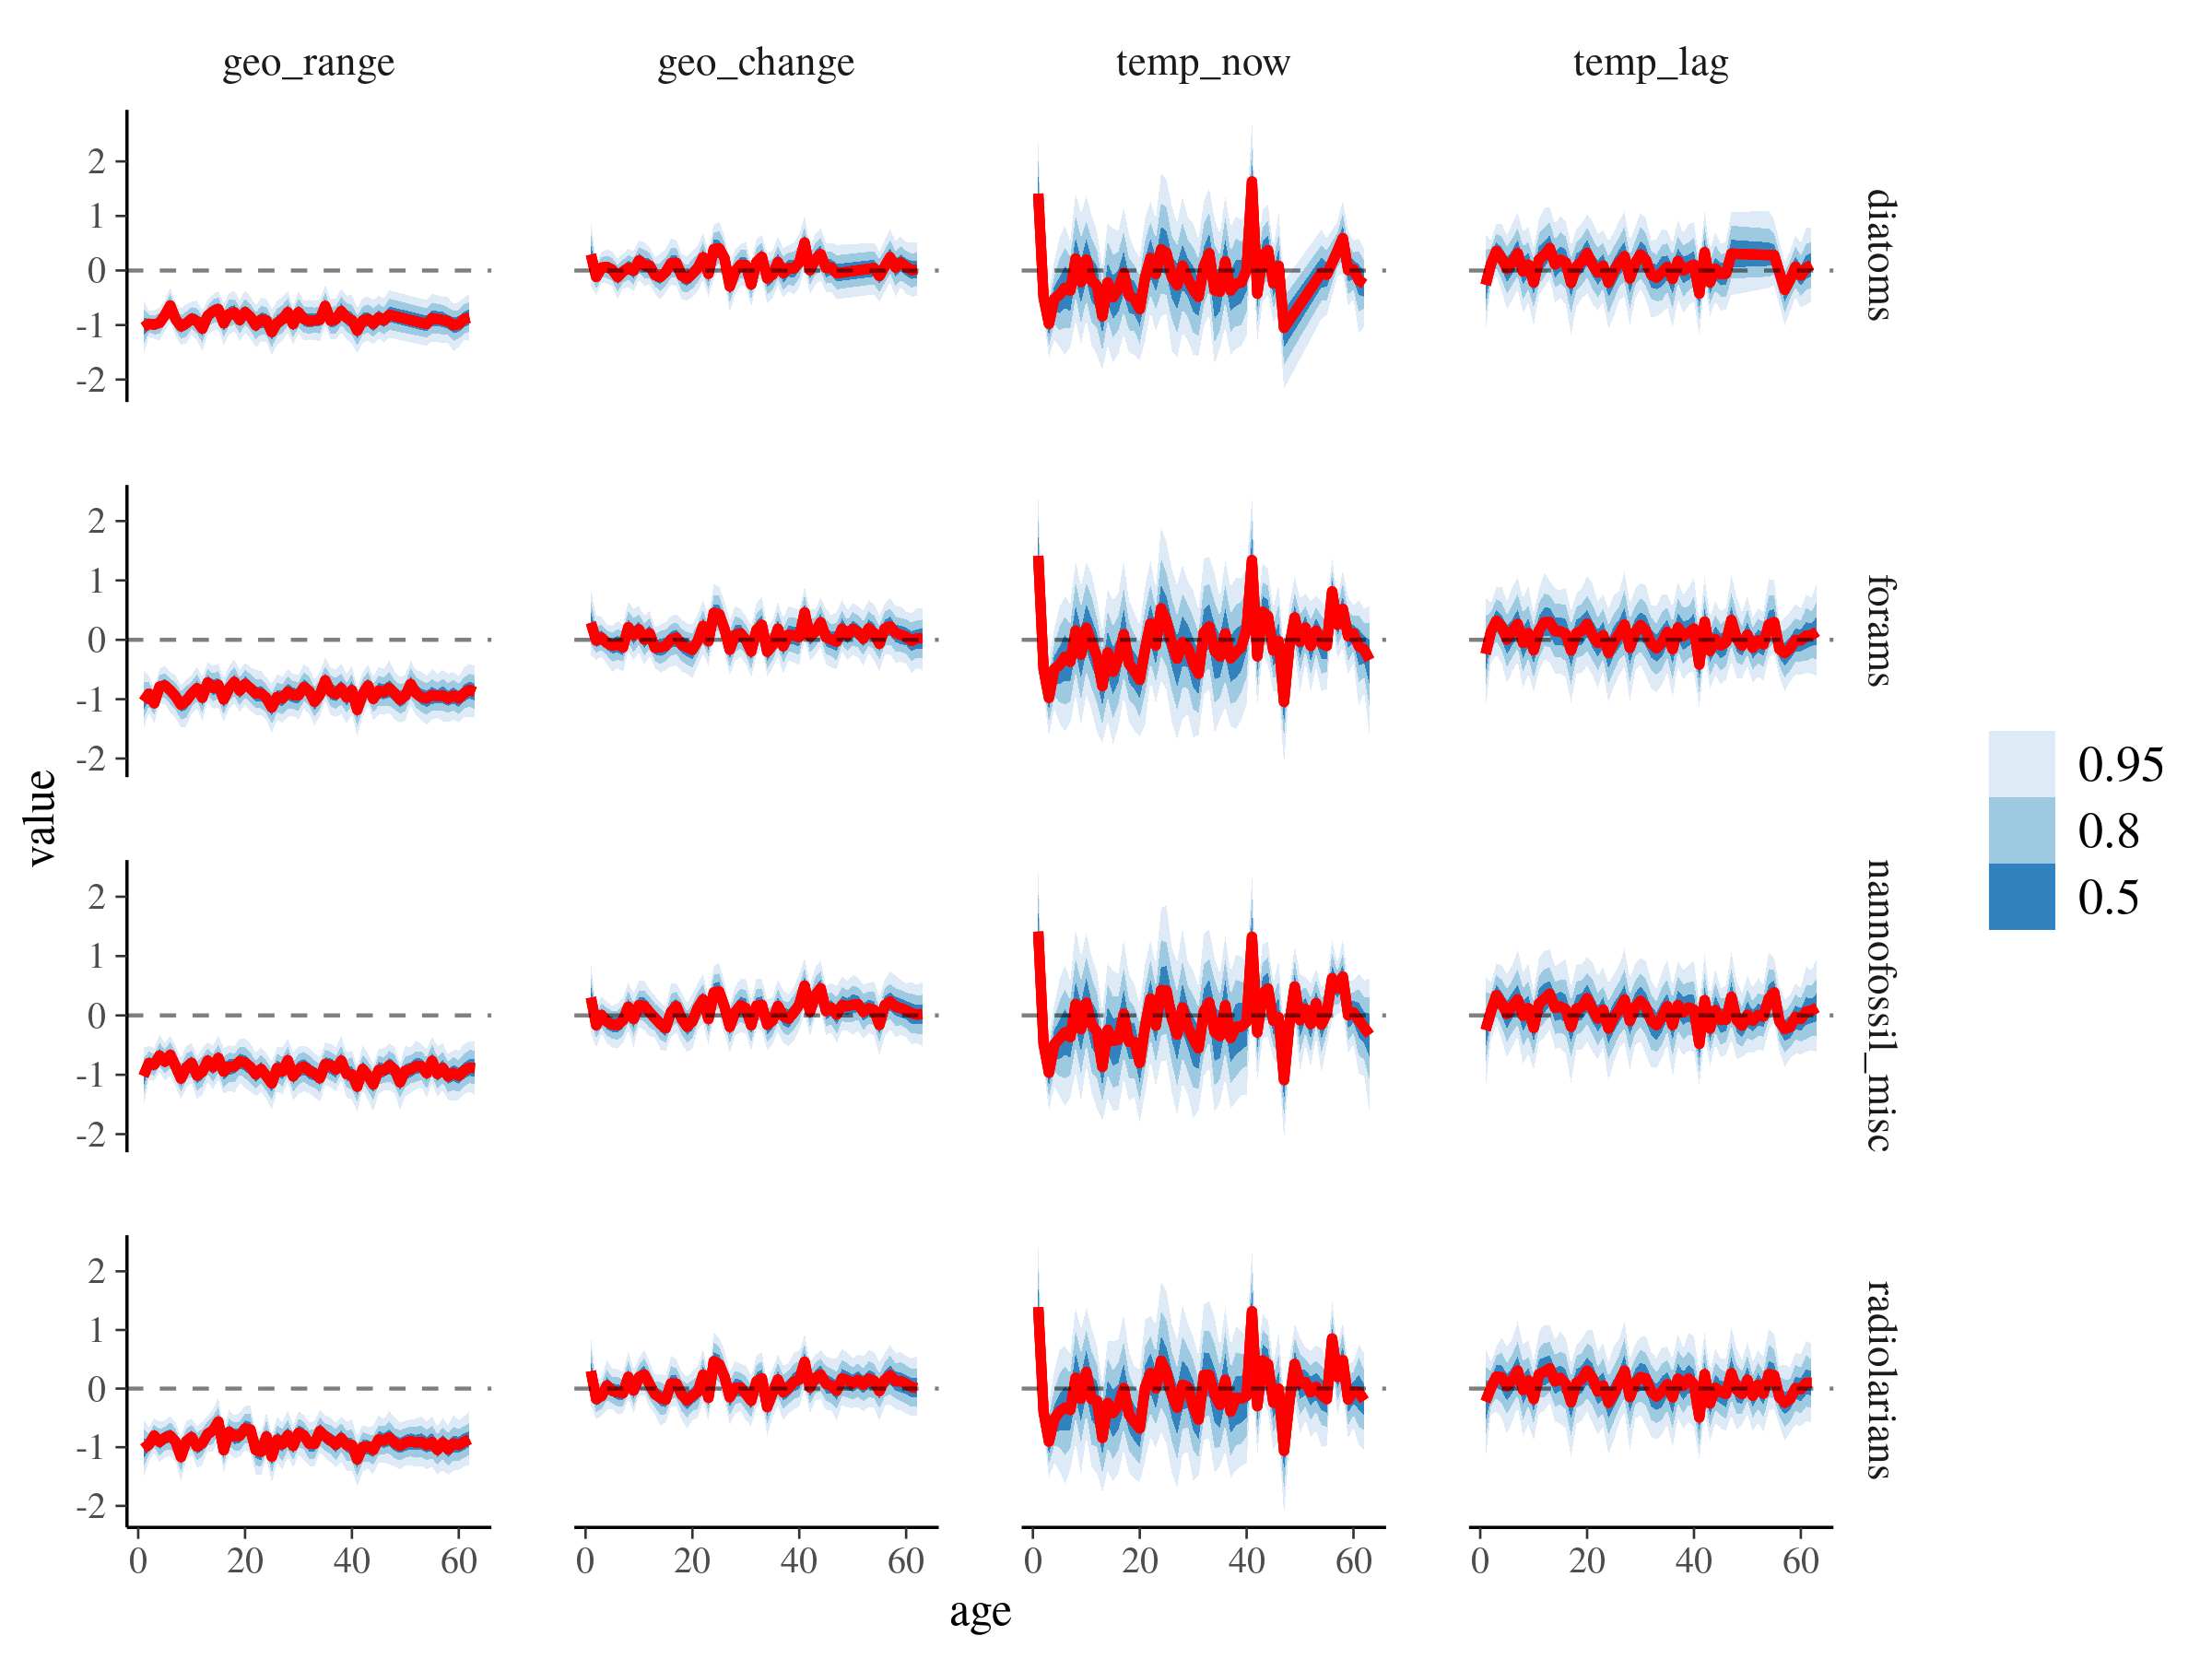
\includegraphics[width=\textwidth,height=0.5\textheight,keepaspectratio=true]{../results/figure/eff_time_group}
%  \caption{Effects of the four covariates as estimated for all time intervals and for each phyla. For each time series, the red line corresponds to the median estimate for each interval, while the envelopes represent various credible intervals as labeled.}
%  \label{fig:effect_time_group}
%\end{figure}
%
%
%% effect of age at observation
%
%% average hazard
%The hazard function describes how age of observation impacts probability of extinction. Hazard is estimated for each phylum for the range of ages observed within the phylum. The matrix \(A\) describes the effect of age on extinction probability for age at observation (rows) by phylum (columns). The phylum-level averages of the effect of age of observation on extinction \(\delta\) are themselves drawn from a distribution centered around 0.
%
%
%Figure \ref{fig:hazard_baseline} is a graph of the average hazard associated with age of observation. This graph illustrates how average extinction risk increases with age for the first few million years before leveling off. A species reaches highest age-related probability of extinction at 10 million years, after which the median becomes volatile until a duration over 30 million years. The flat-ness of the median estimate and the homogeneity of variance durations between approximately 30 million years to under 60 million years is due to the lack of species having survived over 30 million years, which inherently means that these estimates are based on less information and are shrunk towards the overall average while reflecting more and more of our prior uncertainty over time. 
%
%\begin{figure}[ht]
%  \centering
%  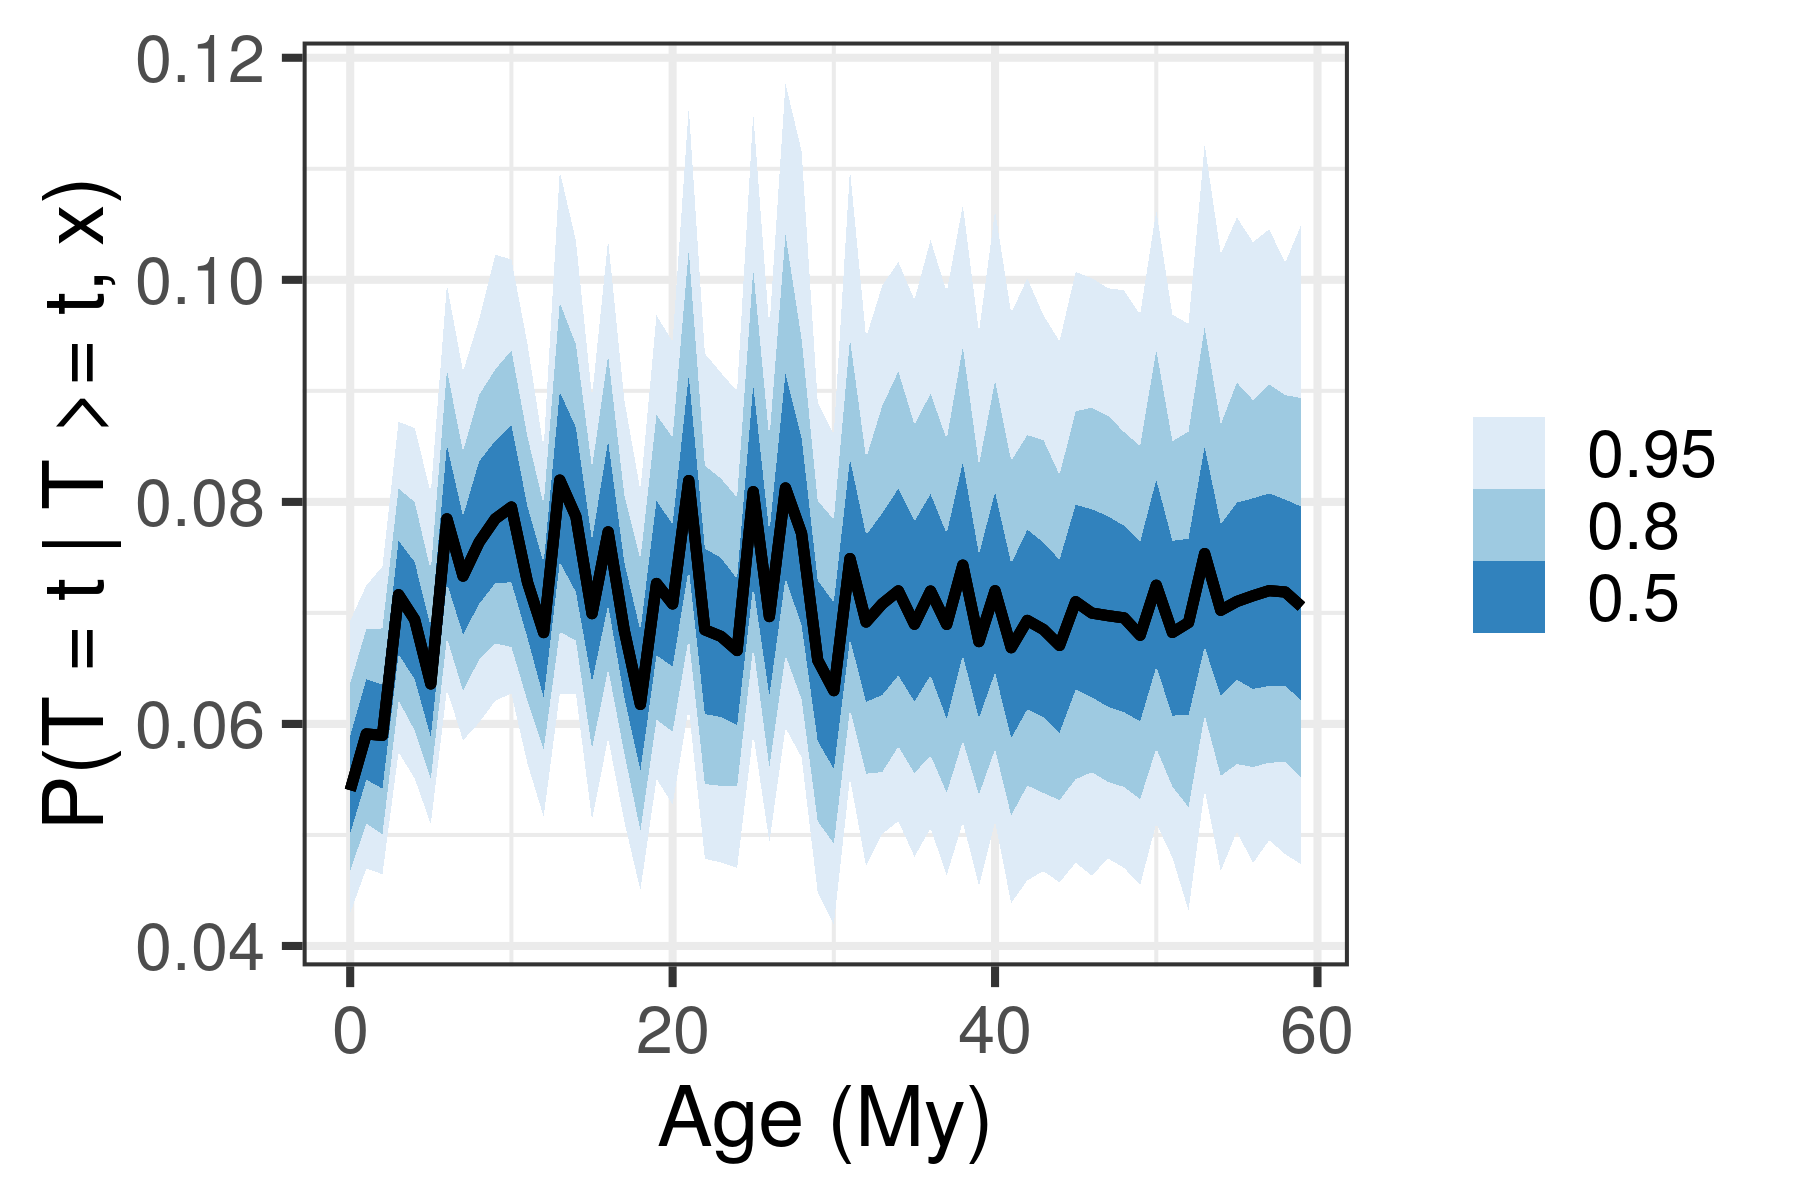
\includegraphics[width=\textwidth,height=0.5\textheight,keepaspectratio=true]{../results/figure/hazard_baseline}
%  \caption{Average hazard estimates based on all all observed species ages in millions of years. Hazard in discrete-survival analysis is the probability of going extinct at a given age having survived up to that age. Overall hazard was calculated using the phylum average intercept and assuming all covariates equaled 0. The red line is the median hazard estimate along with 50\%, 80\%, and 95\% credible intervals.}
%  \label{fig:hazard_baseline}
%\end{figure}
%
%The hazard associated with the individual phyla have broad similarities with the overall hazard estimates (Fig. \ref{fig:hazard_bygroup}). In all four cases, hazard increases over the first 10 million years of a species duration. However, the rate of increase in hazard varies between the phyla, with forams and radiolarians having the most pronounced increase with age. Radiolarians also have the lowest initial hazard of the phyla, followed by forams and calcareous nannoplankton. In contrast, diatoms have the highest initial hazard of the phyla while having the smallest change hazard with age. 
%
%Optimal cutpoint between 0.1 and 0.11 percent. We estimate that the effect of age of observation on extinction can reach this threshold after XX My at YY\% posterior probability.
%
%\begin{figure}[ht]
%  \centering
%  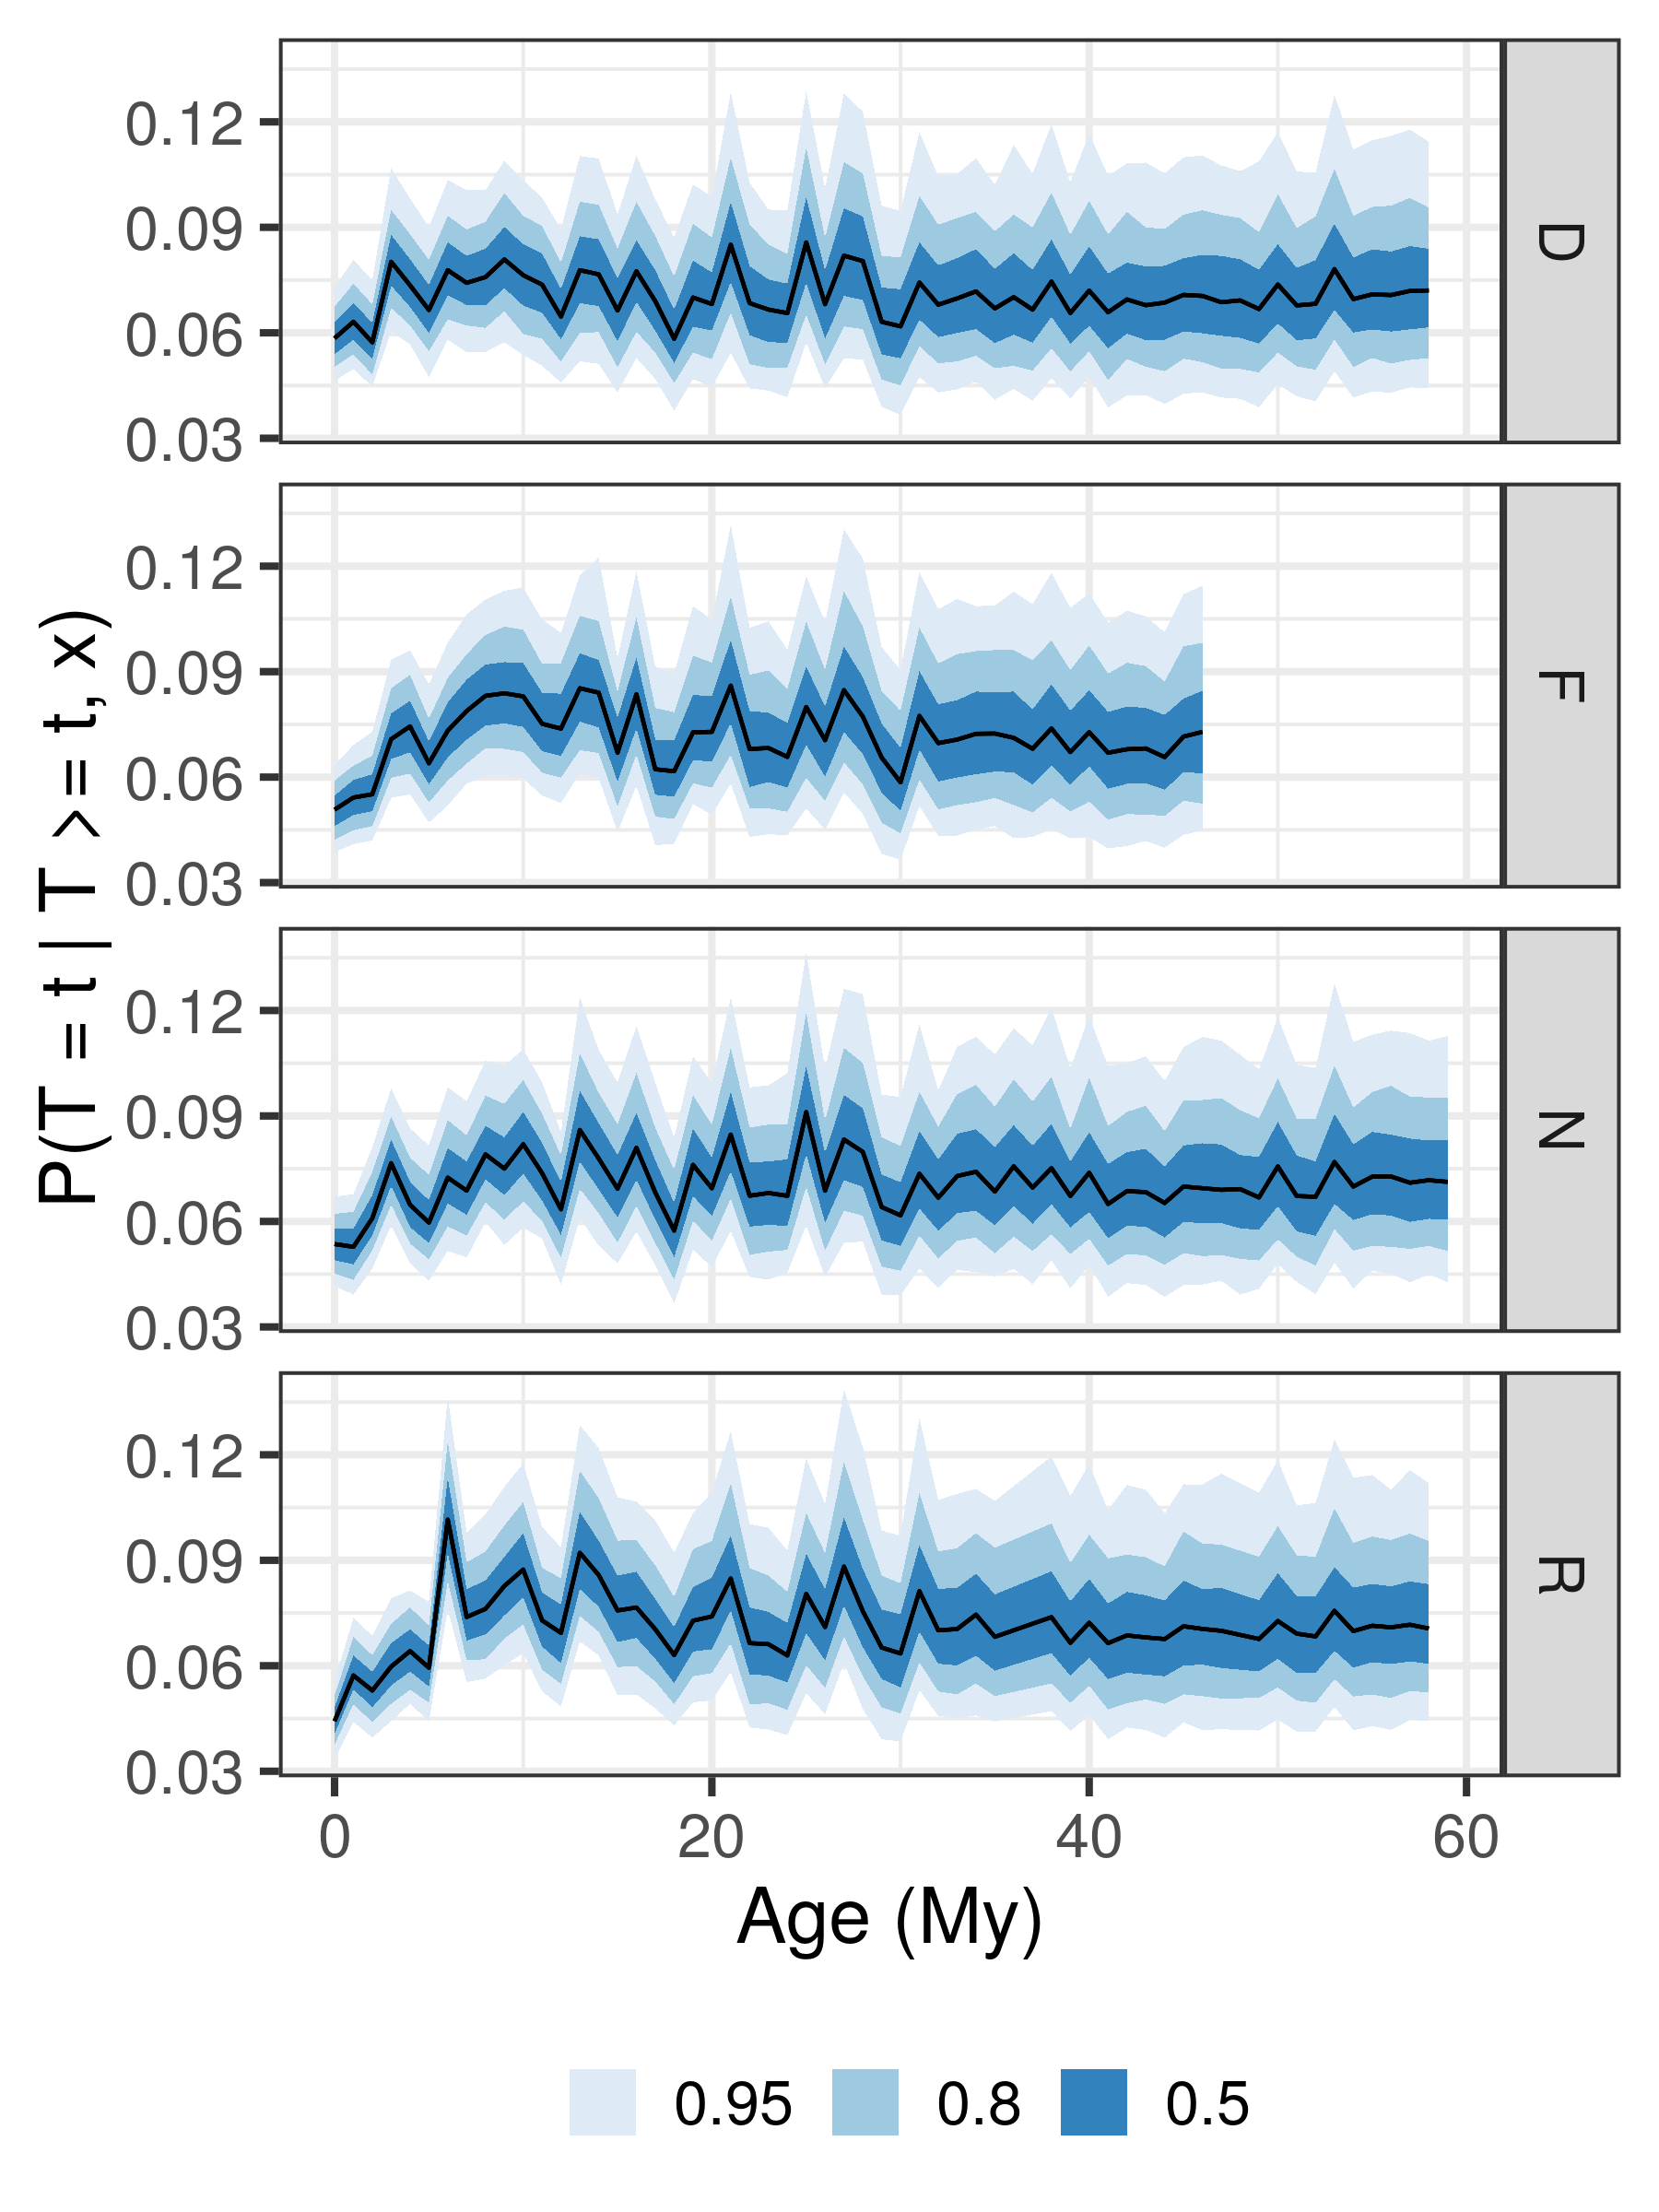
\includegraphics[width=\textwidth,height=0.5\textheight,keepaspectratio=true]{../results/figure/hazard_bygroup}
%  \caption{Hazard estimates for each of the phyla analyzed here. The red line is the median hazard estimate along with 50\%, 80\%, and 95\% credible intervals.}
%  \label{fig:hazard_bygroup}
%\end{figure}
%
%
%% variance components
%There are multiple levels and sources of variance in our model. Each of the grouping factors account for some amount of variance in the data. The first ``level'' of variance is the data level or the variance in the observed data (the model response). In the context of regular linear regression, this variance is equivalent to the residual variance. In the context of logistic regression, however, this value is not an inherent part of the model.
%
%There are then two non-nested sources of the second ``level'' of variance: intercept and slopes varying by time of observation, and a mean-zero age at observation varying intercept. Each of the elements of the vector of scale terms \(\tau_{B}\) describe the within-phyla variance for the intercept and the slope terms for the covariates. Similarly, the scale term \(\sigma_{A}\) is a scalar that describes the within-phyla variance of the effect of age at observation. 
%
%The final ``level'' of variance the phyla-level: the between phyla variance for the intercepts and regression coefficients \(\tau_{\alpha}\), and the between phyla variance for the effect of age at observation \(\sigma_{\delta}\). 
%
%The greatest source of variance accounted for by the grouping factors is the between phylum variance in the model intercept (Fig. \ref{fig:variance_components}); this is the first element of \(\tau_{B}\). All of the other scale terms have approximately equal estimates, which means that they contribute a similar amount to the structure underlying the data. For example, the within-phyla effect of geographic range on extinction probability is associated with approximately as much variance as there is between the phyla themselves.
%
%This result means that, given this model, the greatest contributor to differences in extinction risk over time is when a species is present. In comparison, the covariates we studied individually contribute only a limited amount to the variation in extinction. Similarly, while age at observation does contribute to some differences in extinction risk (Fig XXX age effect), this effect is most likely overwhelmed by the importance of when that observation takes place.
%
%The variance in effects contributed by the phyla is approximately equal to the variance in those effects due to differences over time.
%
%
%\begin{figure}[ht]
%  \centering
%  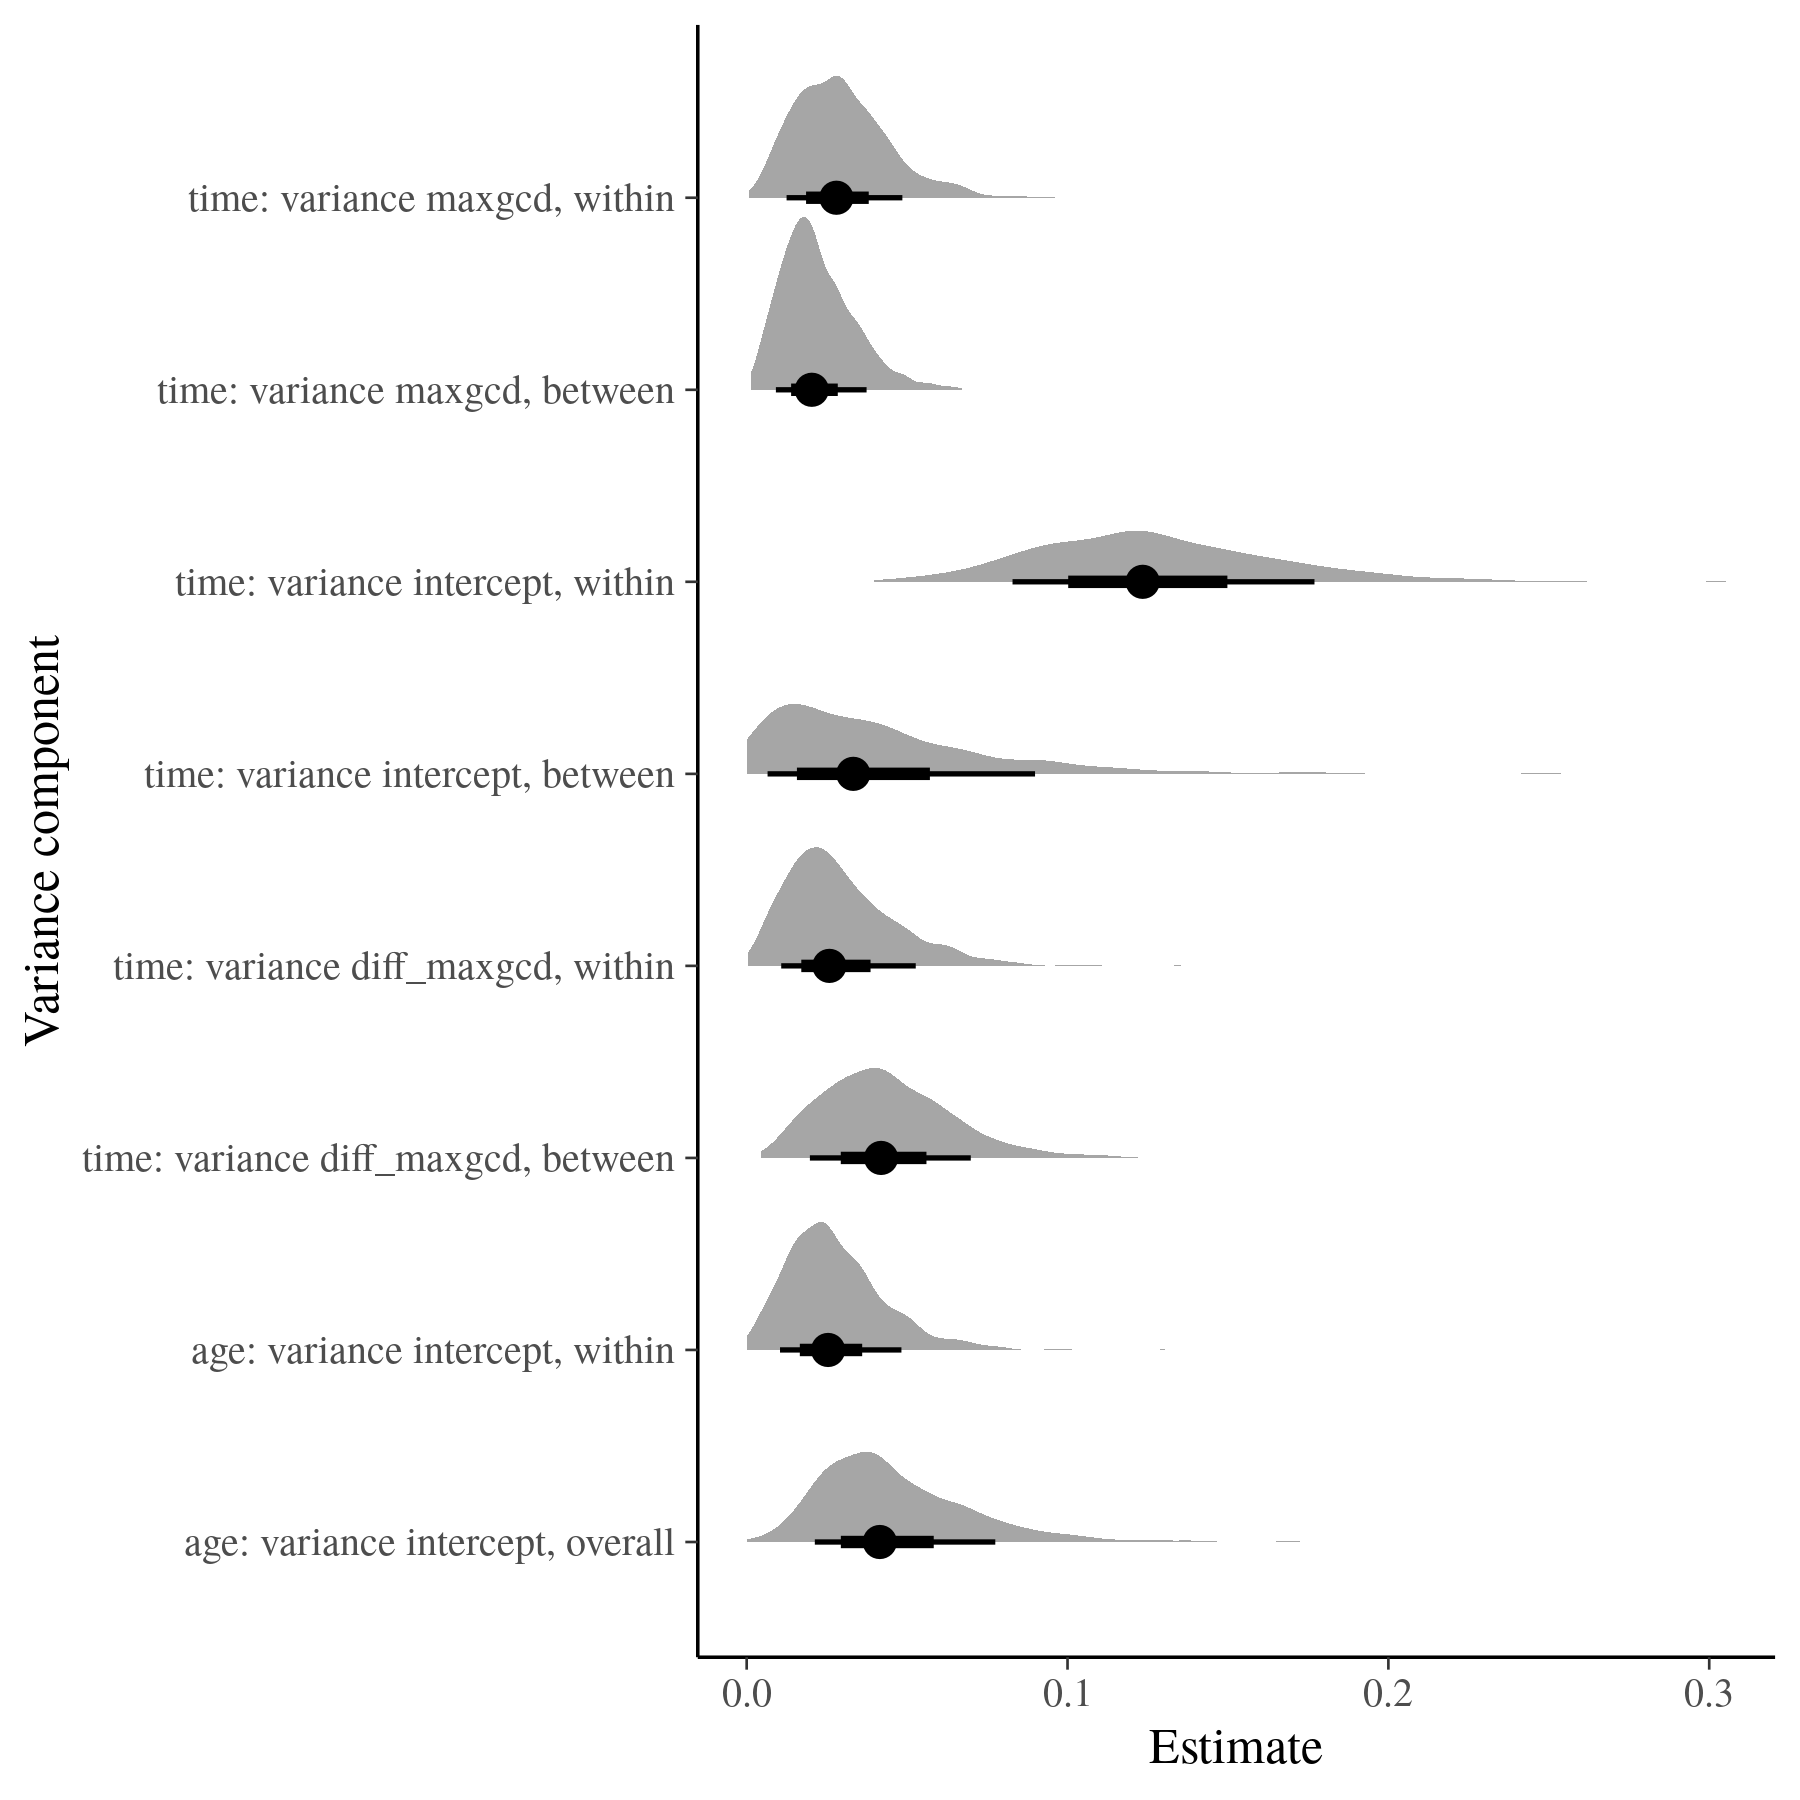
\includegraphics[width=\textwidth,height=0.5\textheight,keepaspectratio=true]{../results/figure/variance_components}
%  \caption{Contribution of multi-level components to unmodeled variance. Larger values indicate a greater contribution to overall variance. Variance components labeled as ``overall'' represent variance between grouping factors, while those labeled  ``within groups'' correspond to variance within grouping factors. If the overall component is greater than the within component, then the groupings do not structure the overall variance. If the within component is greater than the overall component, then the overall variance is structured by the groupings.}
%  \label{fig:variance_components}
%\end{figure}
%
%
%
%Looking at four randomly sampled species, we evaluated their probability of extinction at all times that species was observed. We then compared these estimates to the geographic range trajectory of 
%
%
%% risk estimate compared to change in geo-range
%\begin{figure}[ht]
%  \centering
%  \begin{subfigure}{\textwidth}
%    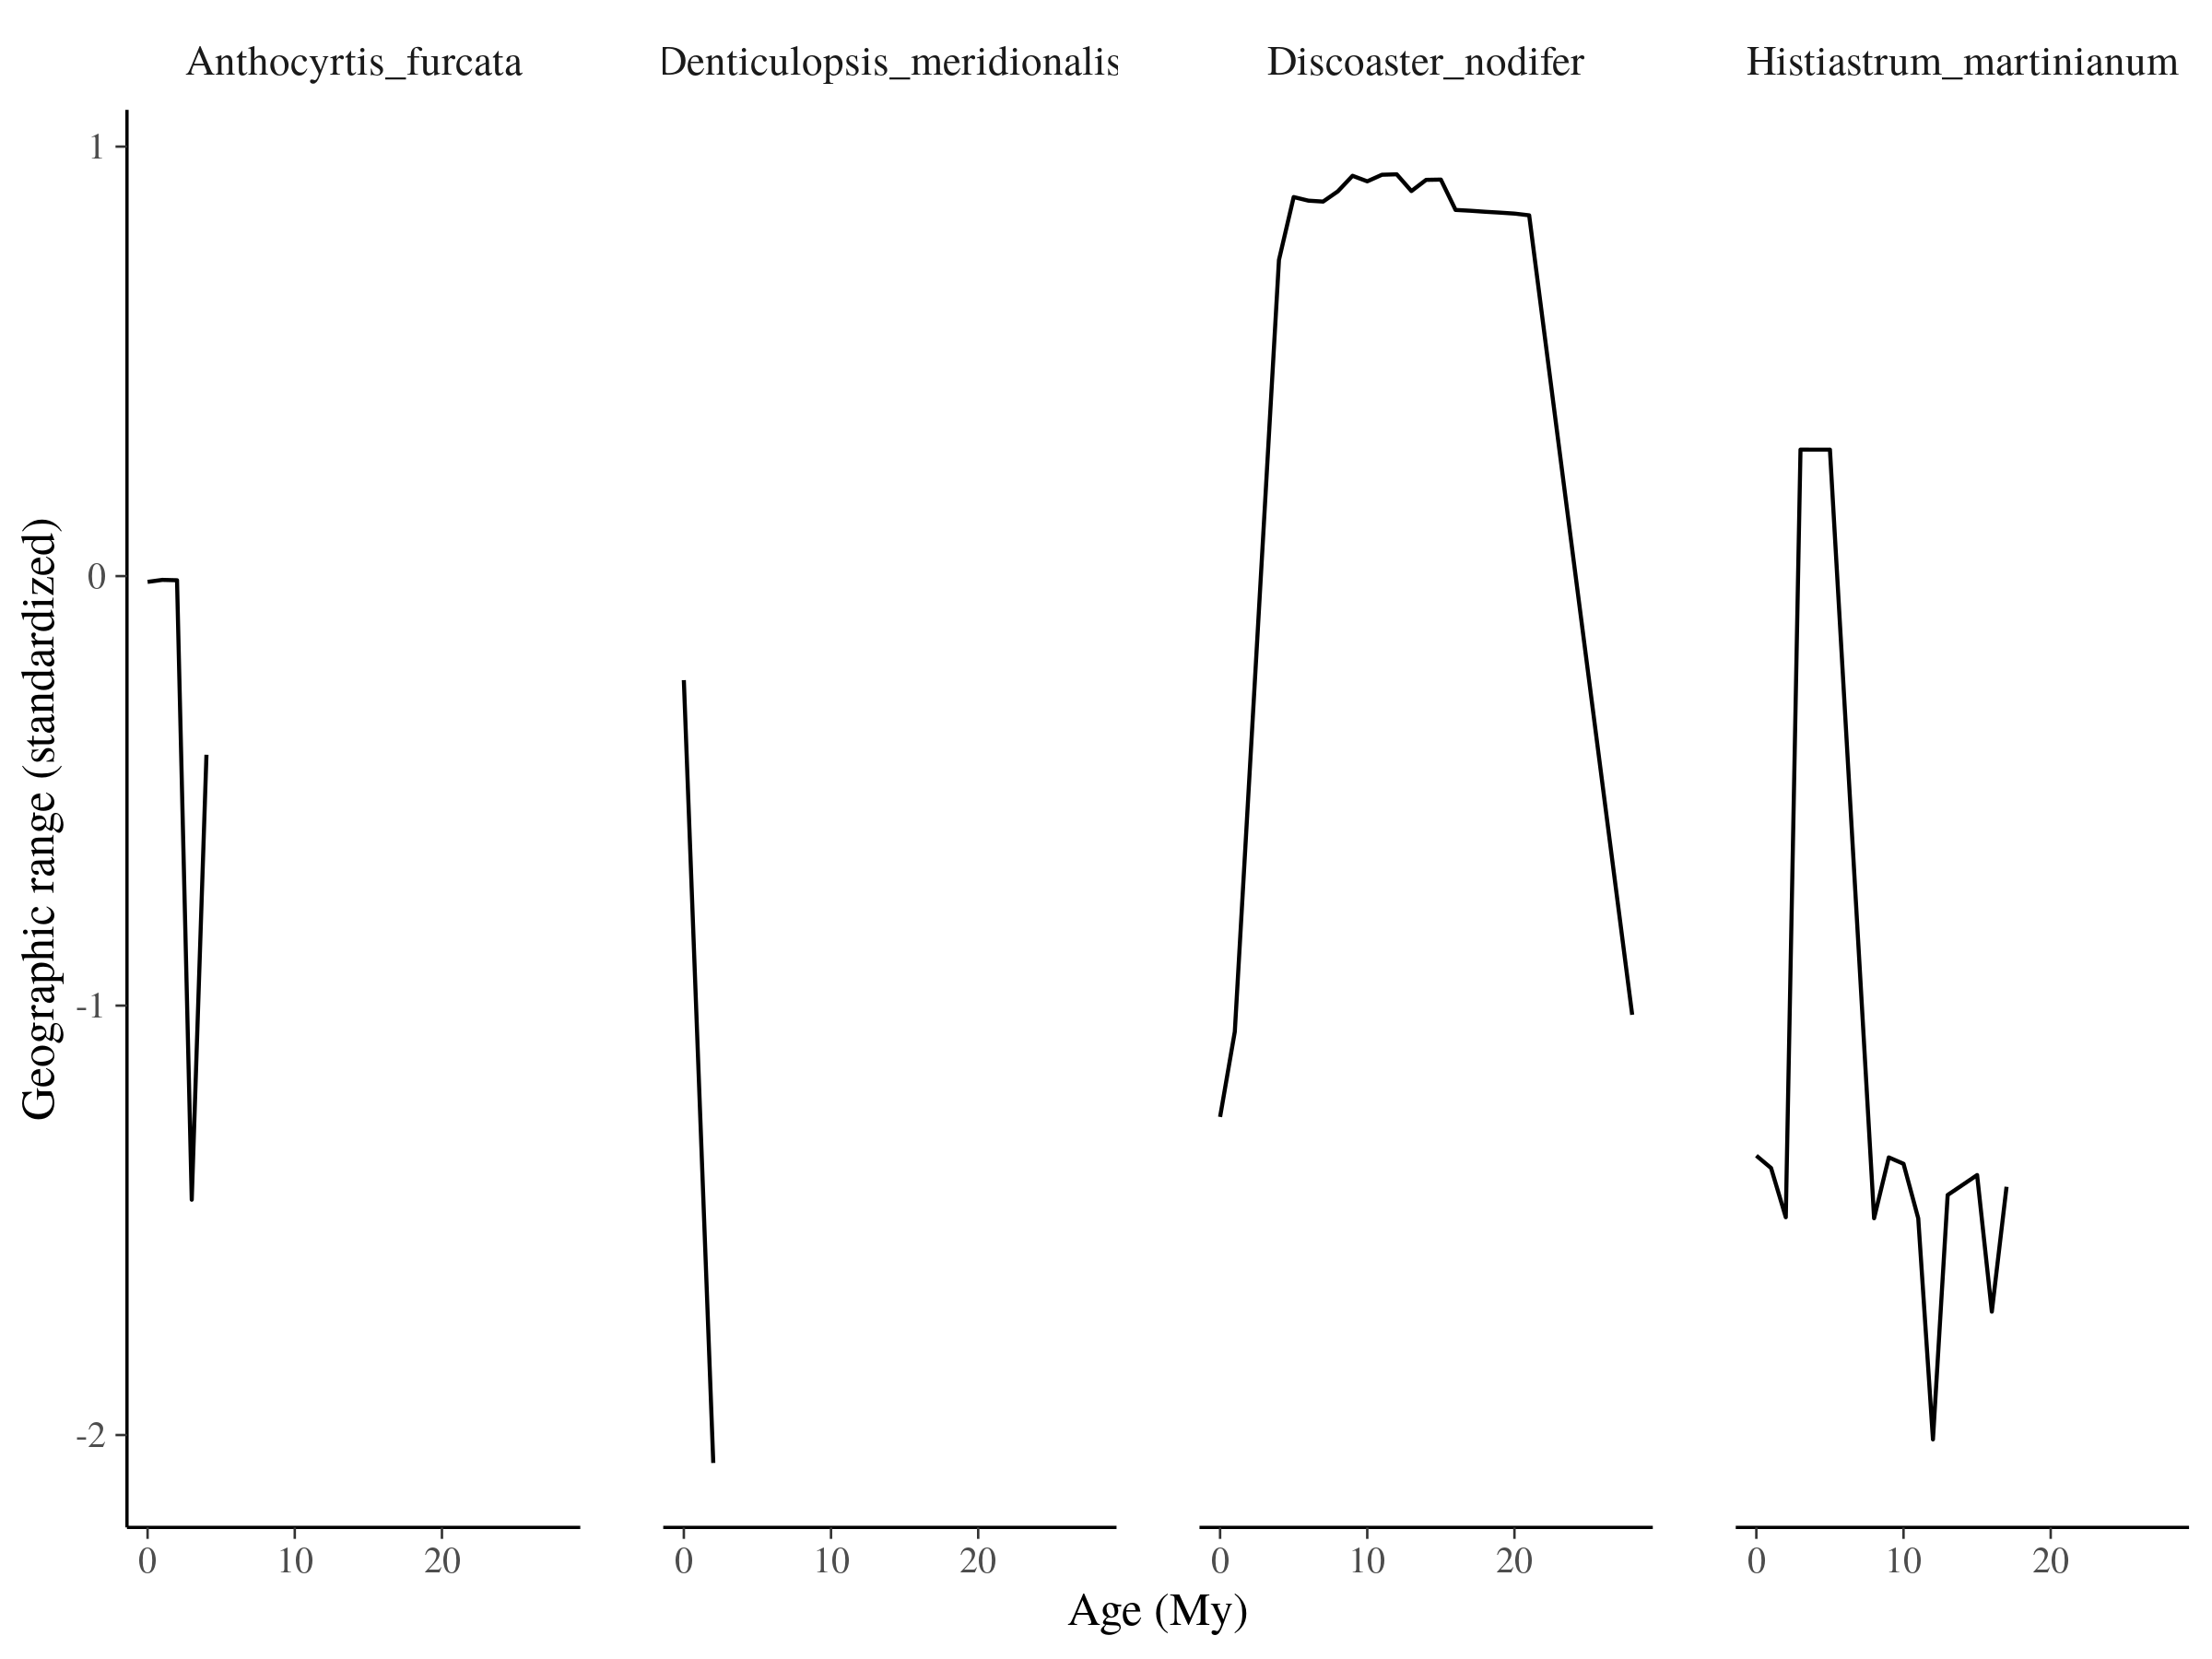
\includegraphics[width=\textwidth,height=0.5\textheight,keepaspectratio=true]{../results/figure/relrisk_range}
%    \caption{A}
%    \label{fig:relrisk_range}
%  \end{subfigure}
%
%  \begin{subfigure}{\textwidth}
%    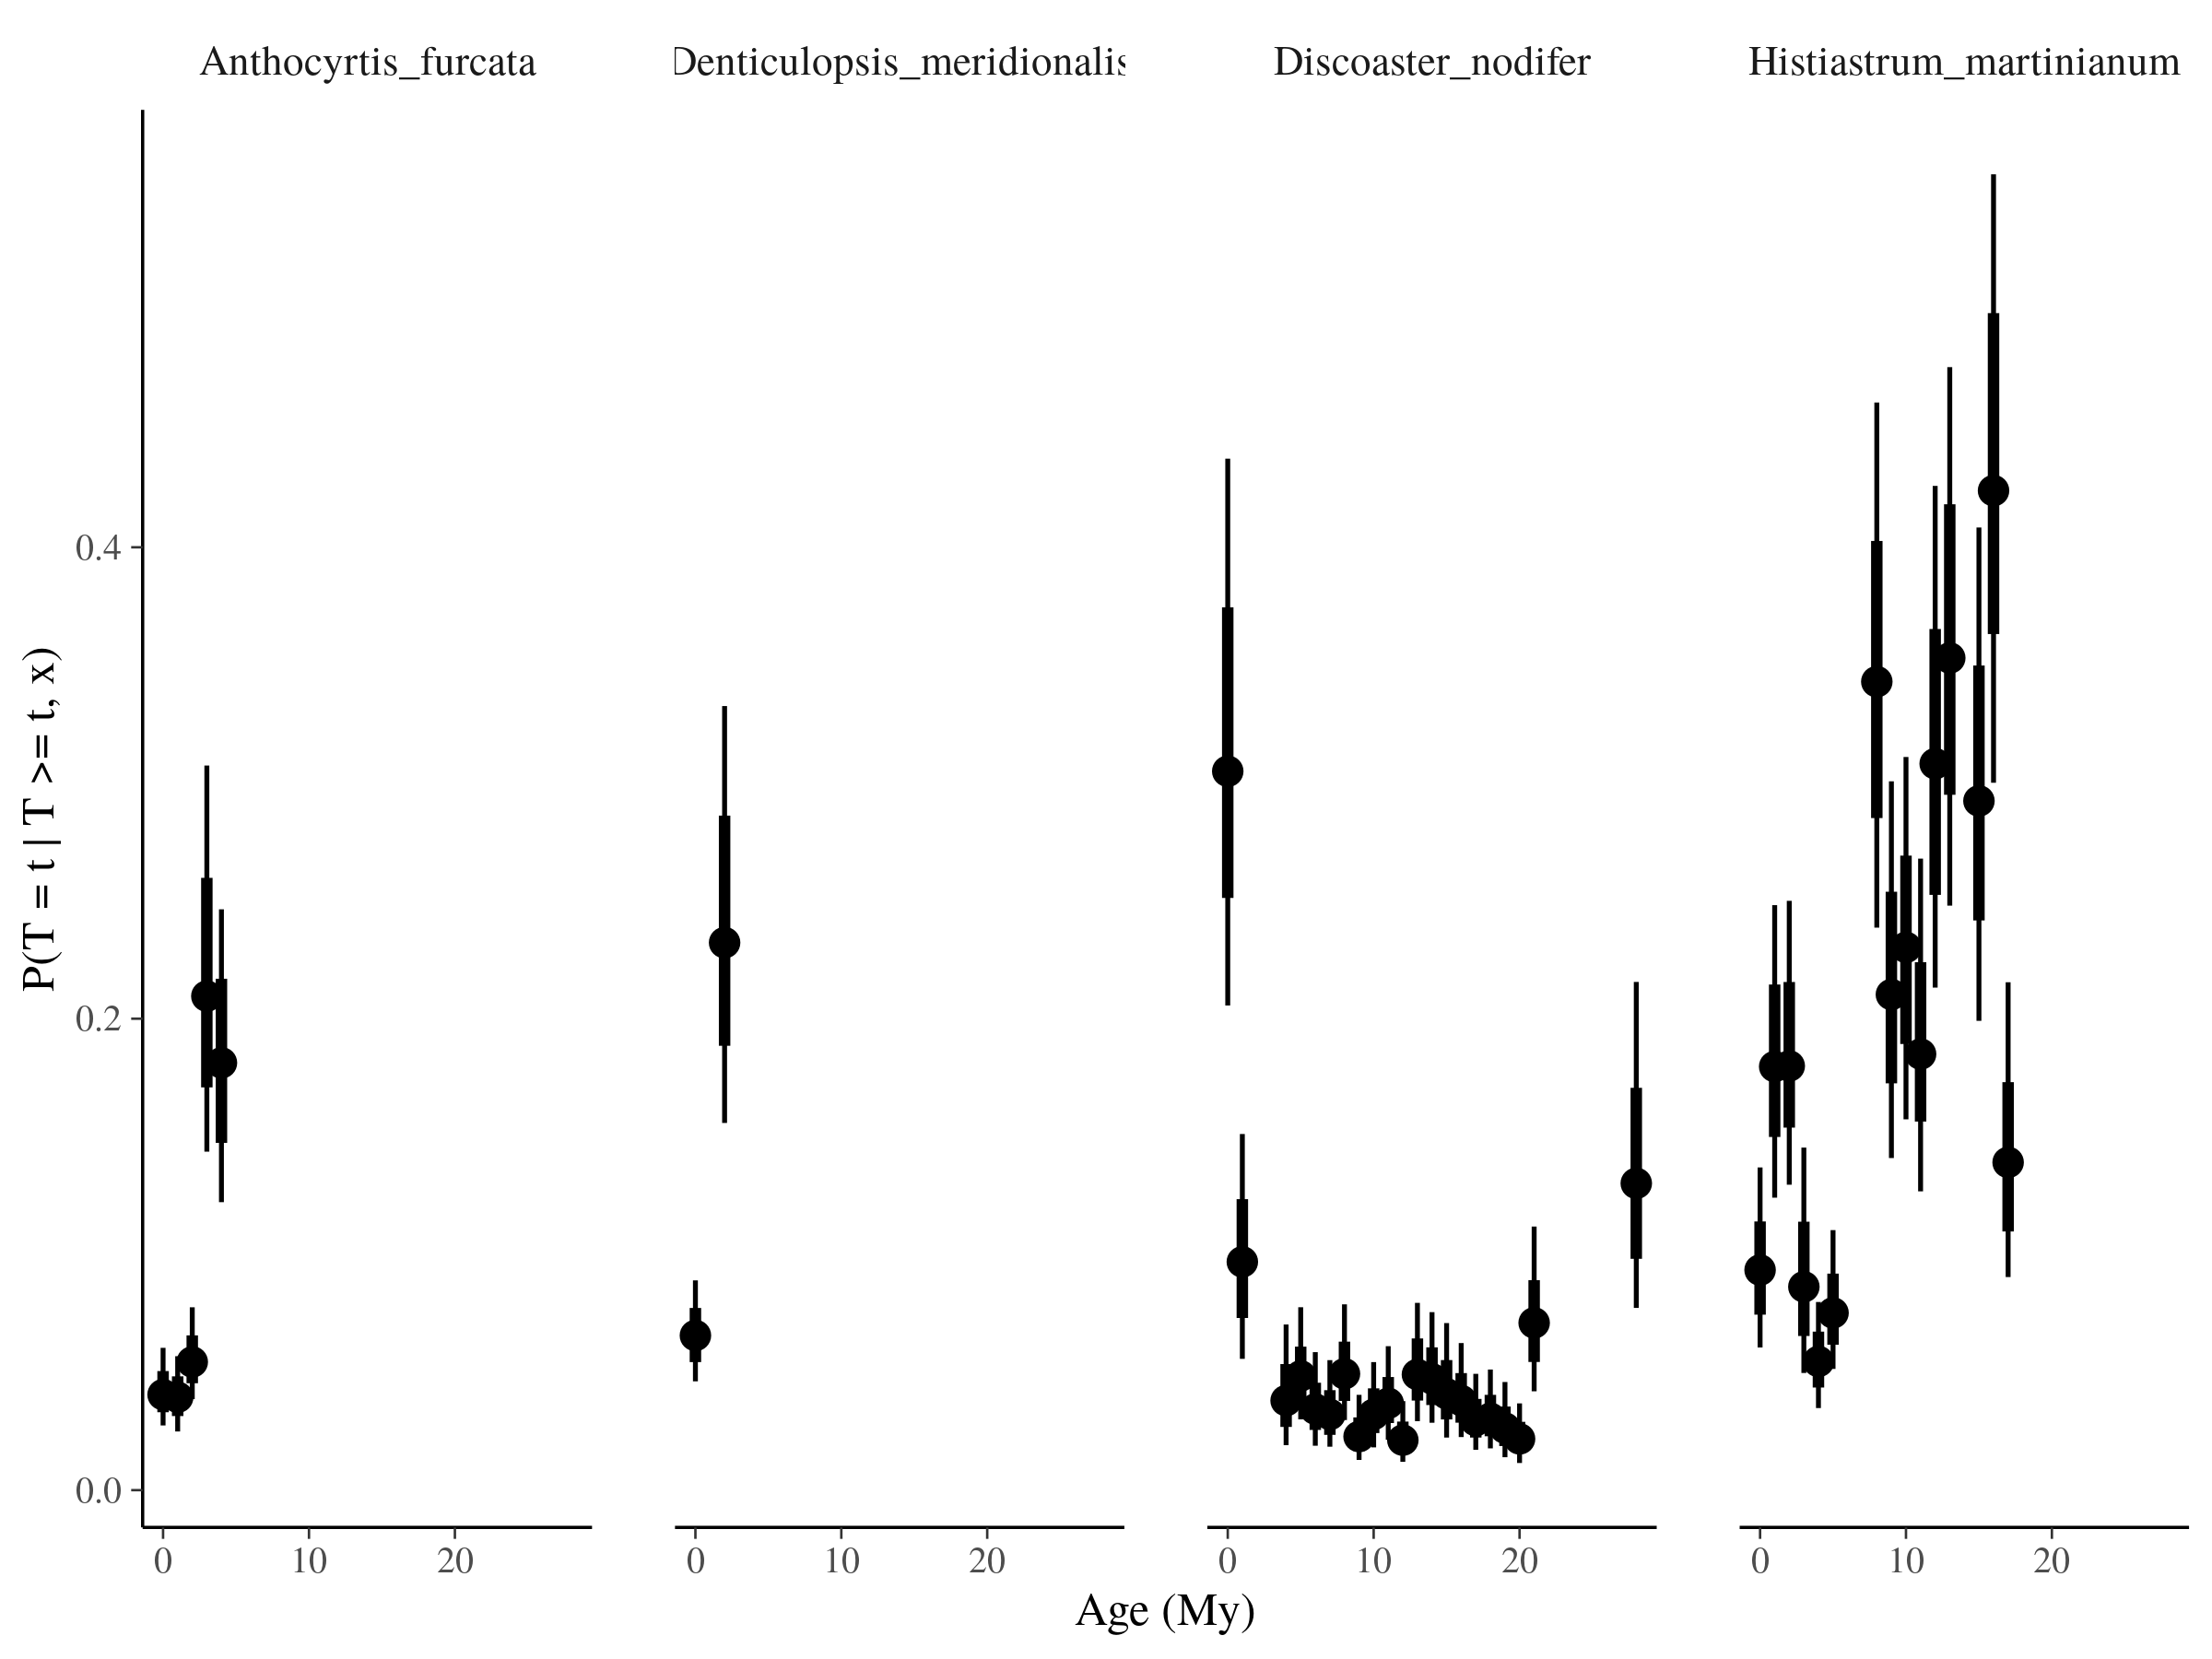
\includegraphics[width=\textwidth,height=0.5\textheight,keepaspectratio=true]{../results/figure/relrisk_ext}
%    \caption{B}
%    \label{fig:relrisk_ext}
%  \end{subfigure}
%  \caption{Comparison between species geogrpahic range histories and our estimate of their probability of extinction for each time of observation. Geographic range is assumed observed without error. Our probability estimates are presented as a median (point) and 50\% and 80\% credible intervals.}
%  \label{fig:relrisk_compare}
%\end{figure}



\end{document}
